\documentclass[10pt,fleqn]{article} % Default font size and left-justified equations
\usepackage[%
    pdftitle={Conception de la commande des systèmes asservis},
    pdfauthor={Xavier Pessoles}]{hyperref}

%%%%%%%%%%%%%%%%%%%%%%%%%%%%%%%%%%%%%%%%%
% Original author:
% Mathias Legrand (legrand.mathias@gmail.com) with modifications by:
% Vel (vel@latextemplates.com)
% License:
% CC BY-NC-SA 3.0 (http://creativecommons.org/licenses/by-nc-sa/3.0/)
%%%%%%%%%%%%%%%%%%%%%%%%%%%%%%%%%%%%%%%%%

%----------------------------------------------------------------------------------------
%	VARIOUS REQUIRED PACKAGES AND CONFIGURATIONS
%----------------------------------------------------------------------------------------

%\usepackage[top=2.5cm,bottom=2cm,left=2cm,right=2cm,headsep=40pt,a4paper]{geometry} % Page margins
\usepackage[top=2cm,bottom=3cm,left=2cm,right=2cm,a4paper]{geometry} % Page margins

\usepackage{graphicx} % Required for including pictures

\usepackage{lipsum} % Inserts dummy text

\usepackage{tikz} % Required for drawing custom shapes

\usepackage[francais]{babel} % English language/hyphenation
\frenchbsetup{StandardLists=true} % Pour éviter la collision babel enumitem pour les listes

\usepackage{enumitem} % Customize lists
\setlist{nolistsep} % Reduce spacing between bullet points and numbered lists

\usepackage{booktabs} % Required for nicer horizontal rules in tables

\usepackage{xcolor} % Required for specifying colors by name
%\definecolor{ocre}{RGB}{243,102,25} % Define the orange color used for highlighting throughout the book
 \definecolor{ocre}{RGB}{49,133,156} % Couleur ''bleue''
\definecolor{violetf}{RGB}{112,48,160} % Couleur ''violet''
\usepackage{enumitem}
\usepackage{pifont} % Pour les dinglist
\usepackage{multicol}
\usepackage{array} % Centrage vertical dans les tableaux
\usepackage{schemabloc}

%----------------------------------------------------------------------------------------
%	FONTS
%----------------------------------------------------------------------------------------
\usepackage{bm}
\usepackage{multicol}
\usepackage{siunitx}
\sisetup{output-decimal-marker = {,}}


\usepackage{avant} % Use the Avantgarde font for headings
%\usepackage{times} % Use the Times font for headings
%\usepackage{mathptmx} % Use the Adobe Times Roman as the default text font together with math symbols from the Sym­bol, Chancery and Com­puter Modern fonts
\usepackage[adobe-utopia]{mathdesign}
\usepackage{microtype} % Slightly tweak font spacing for aesthetics
\usepackage[utf8]{inputenc} % Required for including letters with accents
\usepackage[T1]{fontenc} % Use 8-bit encoding that has 256 glyphs

%----------------------------------------------------------------------------------------
%	BIBLIOGRAPHY AND INDEX
%----------------------------------------------------------------------------------------

%\usepackage[style=alphabetic,citestyle=numeric,sorting=nyt,sortcites=true,autopunct=true,babel=hyphen,hyperref=true,abbreviate=false,backref=true,backend=biber]{biblatex}
\usepackage[style=alphabetic,citestyle=numeric,sorting=nyt,sortcites=true,autopunct=true,hyperref=true,abbreviate=false,backref=true,backend=biber]{biblatex}
\addbibresource{bibliography.bib} % BibTeX bibliography file
\defbibheading{bibempty}{}

\usepackage{calc} % For simpler calculation - used for spacing the index letter headings correctly
\usepackage{makeidx} % Required to make an index
\makeindex % Tells LaTeX to create the files required for indexing

%----------------------------------------------------------------------------------------
%	MAIN TABLE OF CONTENTS
%----------------------------------------------------------------------------------------

\usepackage{titletoc} % Required for manipulating the table of contents

\setcounter{tocdepth}{2}     % Dans la table des matieres
\setcounter{secnumdepth}{2}

\contentsmargin{0cm} % Removes the default margin

% Part text styling
\titlecontents{part}[0cm]
{\addvspace{20pt}\centering\large\bfseries}
{}
{}
{}

% Chapter text styling
\titlecontents{chapter}[1.25cm] % Indentation
{\addvspace{12pt}\large\sffamily\bfseries} % Spacing and font options for chapters
{\color{ocre!60}\contentslabel[\Large\thecontentslabel]{1.25cm}\color{ocre}} % Chapter number
{\color{ocre}}  
{\color{ocre!60}\normalsize\;\titlerule*[.5pc]{.}\;\thecontentspage} % Page number

% Section text styling
\titlecontents{section}[1.25cm] % Indentation
{\addvspace{3pt}\sffamily\bfseries} % Spacing and font options for sections
{\color{ocre!60}\contentslabel[\thecontentslabel]{1.25cm} \color{ocre}} % Section number
{\color{ocre}}
{\hfill\color{ocre!60}\thecontentspage} % Page number
[]

% Subsection text styling
\titlecontents{subsection}[1.25cm] % Indentation
{\addvspace{1pt}\sffamily\small} % Spacing and font options for subsections
{\contentslabel[\thecontentslabel]{1.25cm}} % Subsection number
{}
{\ \titlerule*[.5pc]{.}\;\thecontentspage} % Page number
[]


% Subsection text styling
\titlecontents{subsubsection}[1.25cm] % Indentation
{\addvspace{1pt}\sffamily\small} % Spacing and font options for subsections
{\contentslabel[\thecontentslabel]{1.25cm}} % Subsection number
{}
{\ \titlerule*[.5pc]{.}\;\thecontentspage} % Page number
[]

% List of figures
\titlecontents{figure}[0em]
{\addvspace{-5pt}\sffamily}
{\thecontentslabel\hspace*{1em}}
{}
{\ \titlerule*[.5pc]{.}\;\thecontentspage}
[]

% List of tables
\titlecontents{table}[0em]
{\addvspace{-5pt}\sffamily}
{\thecontentslabel\hspace*{1em}}
{}
{\ \titlerule*[.5pc]{.}\;\thecontentspage}
[]

%----------------------------------------------------------------------------------------
%	MINI TABLE OF CONTENTS IN PART HEADS
%----------------------------------------------------------------------------------------

% Chapter text styling
\titlecontents{lchapter}[0em] % Indenting
{\addvspace{15pt}\large\sffamily\bfseries} % Spacing and font options for chapters
{\color{ocre}\contentslabel[\Large\thecontentslabel]{1.25cm}\color{ocre}} % Chapter number
{}  
{\color{ocre}\normalsize\sffamily\bfseries\;\titlerule*[.5pc]{.}\;\thecontentspage} % Page number

% Section text styling
\titlecontents{lsection}[0em] % Indenting
{\sffamily\small} % Spacing and font options for sections
{\contentslabel[\thecontentslabel]{1.25cm}} % Section number
{}
{}

% Subsection text styling
\titlecontents{lsubsection}[.5em] % Indentation
{\normalfont\footnotesize\sffamily} % Font settings
{}
{}
{}

%----------------------------------------------------------------------------------------
%	PAGE HEADERS
%----------------------------------------------------------------------------------------

\usepackage{fancyhdr} % Required for header and footer configuration



\pagestyle{fancy}
 \renewcommand{\headrulewidth}{0pt}
 \fancyhead{}
 
 % ENTETES de page
 \fancyhead[L]{%
 \noindent\begin{minipage}[c]{2.6cm}%
 
\includegraphics[width=2cm]{logo_lycee.png}%
 \end{minipage}
}

\fancyhead[C]{\rule{8cm}{.5pt}}

 \fancyhead[R]{%
 \noindent\begin{minipage}[c]{3cm}
 \begin{flushright}
 \footnotesize{\textit{\textsf{\xxtete}}}%
 \end{flushright}
 \end{minipage}
}

 \fancyfoot{}
 % PIEDS de page
\fancyfoot[C]{\rule{12cm}{.5pt}}
\renewcommand{\footrulewidth}{0.2pt}
\fancyfoot[C]{\footnotesize{\bfseries \thepage}}
\fancyfoot[L]{ 
\begin{minipage}[c]{.4\linewidth}
\noindent\footnotesize{{\xxauteur}}
\end{minipage}}

\fancyfoot[R]{\footnotesize{\xxpied}
\ifthenelse{\isodd{\value{page}}}{
\begin{tikzpicture}[overlay]
\node[shape=rectangle, 
      rounded corners = .25 cm,
	  draw= ocre,
	  line width=2pt, 
	  fill = ocre!10,
	  minimum width  = 2.5cm,
	  minimum height = 3cm,] at (\xxposongletx,\xxposonglety) {};
\node at (\xxposonglettext,\xxposonglety) {\rotatebox{90}{\textbf{\large\color{ocre}{\xxonglet}}}};
%{};
\end{tikzpicture}}{}
}



%
%
%
% Removes the header from odd empty pages at the end of chapters
\makeatletter
%\renewcommand{\cleardoublepage}{
%\clearpage\ifodd\c@page\else
%\hbox{}
%\vspace*{\fill}
%\thispagestyle{empty}
%\newpage
%\fi}

%\fancypagestyle{plain}{%
%\fancyhf{} % vide l’en-tête et le pied~de~page.
%%\fancyfoot[C]{\bfseries \thepage} % numéro de la page en cours en gras
%% et centré en pied~de~page.
%\fancyfoot[R]{\footnotesize{\xxpied}}
%\fancyfoot[C]{\rule{12cm}{.5pt}}
%\renewcommand{\footrulewidth}{0.2pt}
%\fancyfoot[C]{\footnotesize{\bfseries \thepage}}
%\fancyfoot[L]{ 
%\begin{minipage}[c]{.4\linewidth}
%\noindent\footnotesize{{\xxauteur}}
%\end{minipage}}}

\fancypagestyle{plain}{%
\fancyhf{} % vide l’en-tête et le pied~de~page.
\fancyfoot[C]{\rule{12cm}{.5pt}}
\renewcommand{\footrulewidth}{0.2pt}
\fancyfoot[C]{\footnotesize{\bfseries \thepage}}
\fancyfoot[L]{ 
\begin{minipage}[c]{.4\linewidth}
\noindent\footnotesize{{\xxauteur}}
\end{minipage}}
\fancyfoot[R]{\footnotesize{\xxpied}}
}




%----------------------------------------------------------------------------------------
%	THEOREM STYLES
%----------------------------------------------------------------------------------------

% Conflit avec la police adobe
%\usepackage{amsmath,amsfonts,amssymb,amsthm} % For math equations, theorems, symbols, etc
\usepackage{amsmath,amsthm}

\newcommand{\intoo}[2]{\mathopen{]}#1\,;#2\mathclose{[}}
\newcommand{\ud}{\mathop{\mathrm{{}d}}\mathopen{}}
\newcommand{\intff}[2]{\mathopen{[}#1\,;#2\mathclose{]}}
%\newtheorem{notation}{Notation}[chapter]
\newtheorem{notation}{Notation}[section]

% Boxed/framed environments
\newtheoremstyle{ocrenumbox}% % Theorem style name
{0pt}% Space above
{0pt}% Space below
{\normalfont}% % Body font
{}% Indent amount
{\small\bf\sffamily\color{ocre}}% % Theorem head font
{\;}% Punctuation after theorem head
{0.25em}% Space after theorem head
{\small\sffamily\color{ocre}\thmname{#1}\nobreakspace\thmnumber%{\@ifnotempty{#1}{}\@upn{#2}}% Theorem text (e.g. Theorem 2.1)
\thmnote{\nobreakspace\the\thm@notefont\sffamily\bfseries\color{black}---\nobreakspace#3.}} % Optional theorem note
\renewcommand{\qedsymbol}{$\blacksquare$}% Optional qed square


% Boite pour les corriges
\newtheoremstyle{correctionbox}% % Theorem style name
{0pt}% Space above
{0pt}% Space below
{\normalfont}% % Body font
{}% Indent amount
{\small\bf\sffamily\color{violet}}% % Theorem head font
{\;}% Punctuation after theorem head
{0.25em}% Space after theorem head
{\small\sffamily\color{ocre}\thmname{#1}\nobreakspace\thmnumber%{\@ifnotempty{#1}{}\@upn{#2}}% Theorem text (e.g. Theorem 2.1)
\thmnote{\nobreakspace\the\thm@notefont\sffamily\bfseries\color{black}---\nobreakspace#3.}} % Optional theorem note
\renewcommand{\qedsymbol}{$\blacksquare$}% Optional qed square



\newtheoremstyle{blacknumex}% Theorem style name
{5pt}% Space above
{5pt}% Space below
{\normalfont}% Body font
{} % Indent amount
{\small\bf\sffamily}% Theorem head font
{\;}% Punctuation after theorem head
{0.25em}% Space after theorem head
{\small\sffamily{\tiny\ensuremath{\blacksquare}}\nobreakspace\thmname{#1}\nobreakspace\thmnumber%{\@ifnotempty{#1}{}\@upn{#2}}% Theorem text (e.g. Theorem 2.1)
\thmnote{\nobreakspace\the\thm@notefont\sffamily\bfseries---\nobreakspace#3.}}% Optional theorem note

\newtheoremstyle{blacknumbox} % Theorem style name
{0pt}% Space above
{0pt}% Space below
{\normalfont}% Body font
{}% Indent amount
{\small\bf\sffamily}% Theorem head font
{\;}% Punctuation after theorem head
{0.25em}% Space after theorem head
{\small\sffamily\thmname{#1}\nobreakspace 
\thmnote{\nobreakspace\the\thm@notefont\sffamily\bfseries---\nobreakspace#3.}}% Optional theorem note

% Non-boxed/non-framed environments
\newtheoremstyle{ocrenum}% % Theorem style name
{5pt}% Space above
{5pt}% Space below
{\normalfont}% % Body font
{}% Indent amount
{\small\bf\sffamily\color{ocre}}% % Theorem head font
{\;}% Punctuation after theorem head
{0.25em}% Space after theorem head
{\small\sffamily\color{ocre}\thmname{#1}\nobreakspace%\thmnumber{\@ifnotempty{#1}{}\@upn{#2}}% Theorem text (e.g. Theorem 2.1)
\thmnote{\nobreakspace\the\thm@notefont\sffamily\bfseries\color{black}---\nobreakspace#3.}} % Optional theorem note
\renewcommand{\qedsymbol}{$\blacksquare$}% Optional qed square
\makeatother

% Environnement pour les titres de parties
\newtheoremstyle{partiebox} 
{0pt}% Space above
{0pt}% Space below
{\normalfont}% Body font
{}% Indent amount
{\small\bf\sffamily}% Theorem head font
{\;}% Punctuation after theorem head
{0.25em}% Space after theorem head




% Defines the theorem text style for each type of theorem to one of the three styles above
\newcounter{dummy} 
\numberwithin{dummy}{section}
\theoremstyle{ocrenumbox}
%\newtheorem{theoremeT}[dummy]{Théorème}
\newtheorem{theoremeT}[dummy]{Théorème}
\newtheorem{resultatT}[dummy]{Résultat}
\newtheorem{savoirT}[dummy]{Savoir}
\newtheorem{methodeT}[dummy]{Méthode}
\newtheorem{objectifT}[dummy]{Objectif}
%\newtheorem{problem}{Problem}[chapter]
\newtheorem{problem}{Problem}[section]
%\newtheorem{exerciseT}{Exercise}[chapter]
\newtheorem{exerciseT}{Exercice}[section]

\theoremstyle{blacknumex}
%\newtheorem{exampleT}{Example}[chapter]
\newtheorem{exempleT}{Exemple}[section]
\newtheorem{termT}{Terminal\\}[section]
\newtheorem{pyT}{Python\\}[section]
\newtheorem{sciT}{Scilab\\}[section]
\newtheorem{pseudoT}{Pseudo Code\\}[section]
\newtheorem{sqlT}{SQL\\}[section]

\theoremstyle{blacknumbox}
%\newtheorem{vocabulary}{Vocabulary}[chapter]
\newtheorem{vocabulary}{Vocabulaire}[section]
%\newtheorem{definitionT}{Definition}[section]
\newtheorem{definitionT}{Définition}[section]
\newtheorem{rappelT}{Rappel}[section]
\newtheorem{demoT}{Démonstration}[section]
\newtheorem{corollaryT}[dummy]{Corollaire}
\newtheorem{hypoT}{Hypothèse(s)}

\theoremstyle{ocrenum}
\newtheorem{proposition}[dummy]{Proposition}

\theoremstyle{partiebox}
\newtheorem{titrepartieT}[]{}
\newtheorem{titrechapitreT}[]{}

\theoremstyle{correctionbox}
\newtheorem{correctionT}[dummy]{\color{violet}{Correction}}

%----------------------------------------------------------------------------------------
%	DEFINITION OF COLORED BOXES
%----------------------------------------------------------------------------------------

\RequirePackage[framemethod=tikz]{mdframed} % Required for creating the theorem, definition, exercise and corollary boxes

% Theorem box
\newmdenv[skipabove=7pt,
skipbelow=7pt,
backgroundcolor=ocre!10,
linecolor=ocre,
innerleftmargin=5pt,
innerrightmargin=5pt,
innertopmargin=5pt,
leftmargin=0cm,
rightmargin=0cm,
innerbottommargin=5pt]{tBox}


% Correction
\newmdenv[skipabove=7pt,
skipbelow=7pt,
backgroundcolor=violet!10,
linecolor=violet,
innerleftmargin=5pt,
innerrightmargin=5pt,
innertopmargin=5pt,
leftmargin=0cm,
rightmargin=0cm,
innerbottommargin=5pt]{coBox}


% Exercise box	  
\newmdenv[skipabove=7pt,
skipbelow=7pt,
rightline=false,
leftline=true,
topline=false,
bottomline=false,
backgroundcolor=ocre!10,
linecolor=ocre,
innerleftmargin=5pt,
innerrightmargin=5pt,
innertopmargin=5pt,
innerbottommargin=5pt,
leftmargin=0cm,
rightmargin=0cm,
linewidth=4pt]{eBox}	

% Definition box
\newmdenv[skipabove=7pt,
skipbelow=7pt,
rightline=false,
leftline=true,
topline=false,
bottomline=false,
backgroundcolor=ocre!10,
linecolor=ocre,
innerleftmargin=5pt,
innerrightmargin=5pt,
innertopmargin=0pt,
leftmargin=0cm,
rightmargin=0cm,
linewidth=4pt,
innerbottommargin=0pt]{dBox}	

% Demonstration box
\newmdenv[skipabove=7pt,
skipbelow=7pt,
rightline=false,
leftline=true,
topline=false,
bottomline=false,
%backgroundcolor=ocre!10,
linecolor=ocre,
innerleftmargin=5pt,
innerrightmargin=5pt,
innertopmargin=0pt,
leftmargin=0cm,
rightmargin=0cm,
linewidth=4pt,
innerbottommargin=0pt]{demoBox}	

% Corollary box
\newmdenv[skipabove=7pt,
skipbelow=7pt,
rightline=false,
leftline=true,
topline=false,
bottomline=false,
linecolor=gray,
backgroundcolor=black!5,
innerleftmargin=5pt,
innerrightmargin=5pt,
innertopmargin=5pt,
leftmargin=0cm,
rightmargin=0cm,
linewidth=4pt,
innerbottommargin=5pt]{cBox}


% Hypothèses
\newmdenv[skipabove=7pt,
skipbelow=7pt,
rightline=false,
leftline=true,
topline=false,
bottomline=false,
linecolor=gray,
backgroundcolor=black!5,
innerleftmargin=5pt,
innerrightmargin=5pt,
innertopmargin=5pt,
leftmargin=0cm,
rightmargin=0cm,
linewidth=4pt,
innerbottommargin=5pt]{hyBox}


% Boite pour le titre de la partie (pBox)
\newmdenv[skipabove=7pt,
skipbelow=7pt,
rightline=true,
leftline=false,
topline=false,
bottomline=false,
linecolor=ocre,
backgroundcolor=none,
innerleftmargin=5pt,
innerrightmargin=5pt,
innertopmargin=5pt,
leftmargin=0cm,
rightmargin=0cm,
linewidth=4pt,
innerbottommargin=5pt]{pBox}

% Boite pour le titre du chapitre (chBox)
\newmdenv[skipabove=7pt,
skipbelow=7pt,
rightline=false,
leftline=true,
topline=false,
bottomline=false,
linecolor=ocre,
%backgroundcolor=black!5,
innerleftmargin=5pt,
innerrightmargin=5pt,
innertopmargin=5pt,
leftmargin=0cm,
rightmargin=0cm,
linewidth=4pt,
innerbottommargin=5pt]{chBox}


% Boite pour les exemples
\newmdenv[skipabove=7pt,
skipbelow=7pt,
rightline=false,
leftline=true,
topline=false,
bottomline=false,
linecolor=gray,
backgroundcolor=white,
innerleftmargin=5pt,
innerrightmargin=5pt,
innertopmargin=5pt,
leftmargin=0cm,
rightmargin=0cm,
linewidth=4pt,
innerbottommargin=5pt]{exBox}

% Boite pour le terminal
\newmdenv[skipabove=7pt,
skipbelow=7pt,
rightline=false,
leftline=true,
topline=false,
bottomline=false,
linecolor=gray,
backgroundcolor=white,
innerleftmargin=5pt,
innerrightmargin=5pt,
innertopmargin=5pt,
leftmargin=0cm,
rightmargin=0cm,
linewidth=4pt,
innerbottommargin=5pt]{termBox}


% Boite pour Python
\newmdenv[skipabove=7pt,
skipbelow=7pt,
rightline=false,
leftline=true,
topline=false,
bottomline=false,
linecolor=gray,
backgroundcolor=white,
innerleftmargin=5pt,
innerrightmargin=5pt,
innertopmargin=0pt,
leftmargin=0cm,
rightmargin=0cm,
linewidth=4pt,
innerbottommargin=5pt]{pyBox}

% Boite pour scilab
\newmdenv[skipabove=7pt,
skipbelow=7pt,
rightline=false,
leftline=true,
topline=false,
bottomline=false,
linecolor=gray,
backgroundcolor=white,
innerleftmargin=5pt,
innerrightmargin=5pt,
innertopmargin=5pt,
leftmargin=0cm,
rightmargin=0cm,
linewidth=4pt,
innerbottommargin=5pt]{sciBox}


% Boite pour pseudo
\newmdenv[skipabove=7pt,
skipbelow=7pt,
rightline=false,
leftline=true,
topline=false,
bottomline=false,
linecolor=gray,
backgroundcolor=white,
innerleftmargin=5pt,
innerrightmargin=5pt,
innertopmargin=5pt,
leftmargin=0cm,
rightmargin=0cm,
linewidth=4pt,
innerbottommargin=5pt]{pseudoBox}

% Boite pour pseudo
\newmdenv[skipabove=7pt,
skipbelow=7pt,
rightline=false,
leftline=true,
topline=false,
bottomline=false,
linecolor=gray,
backgroundcolor=white,
innerleftmargin=5pt,
innerrightmargin=5pt,
innertopmargin=5pt,
leftmargin=0cm,
rightmargin=0cm,
linewidth=4pt,
innerbottommargin=5pt]{sqlBox}


% Creates an environment for each type of theorem and assigns it a theorem text style from the "Theorem Styles" section above and a colored box from above
\newenvironment{theorem}{\begin{tBox}\begin{theoremeT}}{\end{theoremeT}\end{tBox}}
\newenvironment{resultat}{\begin{tBox}\begin{resultatT}}{\end{resultatT}\end{tBox}}
\newenvironment{methode}{\begin{tBox}\begin{methodeT}}{\end{methodeT}\end{tBox}}
\newenvironment{savoir}{\begin{tBox}\begin{savoirT}}{\end{savoirT}\end{tBox}}
\newenvironment{obj}{\begin{tBox}\begin{objectifT}}{\end{objectifT}\end{tBox}}
\newenvironment{corrige}{\begin{coBox}\begin{correctionT}}{\end{correctionT}\end{coBox}}
\newenvironment{exercise}{\begin{eBox}\begin{exerciseT}}{\hfill{\color{ocre}\tiny\ensuremath{\blacksquare}}\end{exerciseT}\end{eBox}}				  
\newenvironment{exercice}{\begin{eBox}\begin{exerciseT}}{\hfill{\color{ocre}\tiny\ensuremath{\blacksquare}}\end{exerciseT}\end{eBox}}				  

\newenvironment{definition}{\begin{dBox}\begin{definitionT}}{\end{definitionT}\end{dBox}}	
\newenvironment{rappel}{\begin{dBox}\begin{rappelT}}{\end{rappelT}\end{dBox}}	
\newenvironment{defi}{\begin{dBox}\begin{definitionT}}{\end{definitionT}\end{dBox}}	
\newenvironment{demo}{\begin{demoBox}\begin{demoT}}{\end{demoT}\end{demoBox}}	
%\newenvironment{exemple}{\begin{exempleT}}{\hfill{\tiny\ensuremath{\blacksquare}}\end{exempleT}}		
\newenvironment{corollary}{\begin{cBox}\begin{corollaryT}}{\end{corollaryT}\end{cBox}}
\newenvironment{hypo}{\begin{hyBox}\begin{hypoT}}{\end{hypoT}\end{hyBox}}	\newenvironment{exemple}{\begin{exBox}\begin{exempleT}}{\hfill{\tiny\ensuremath{\blacksquare}}\end{exempleT}\end{exBox}}	
\newenvironment{titrepartie}{\begin{pBox}\begin{titrepartieT}}{\end{titrepartieT}\end{pBox}}	
\newenvironment{titrechapitre}{\begin{chBox}\begin{titrechapitreT}}{\end{titrechapitreT}\end{chBox}}	

\newenvironment{term}{ \begin{termBox}\begin{termT}}{\end{termT}\end{termBox}}
\newenvironment{py}{ \begin{pyBox}\begin{pyT}}{\end{pyT}\end{pyBox}}
\newenvironment{sci}{ \begin{sciBox}\begin{sciT}}{\end{sciT}\end{sciBox}}
\newenvironment{pseudo}{ \begin{pseudoBox}\begin{pseudoT}}{\end{pseudoT}\end{pseudoBox}}
\newenvironment{envsql}{ \begin{sqlBox}\begin{sqlT}}{\end{sqlT}\end{sqlBox}}


%----------------------------------------------------------------------------------------
%	REMARK ENVIRONMENT
%----------------------------------------------------------------------------------------

\newenvironment{remark}{\par\vspace{10pt}\small % Vertical white space above the remark and smaller font size
\begin{list}{}{
\leftmargin=35pt % Indentation on the left
\rightmargin=25pt}\item\ignorespaces % Indentation on the right
\makebox[-2.5pt]{\begin{tikzpicture}[overlay]
\node[draw=ocre!60,line width=1pt,circle,fill=ocre!25,font=\sffamily\bfseries,inner sep=2pt,outer sep=0pt] at (-15pt,0pt){\textcolor{ocre}{R}};\end{tikzpicture}} % Orange R in a circle
\advance\baselineskip -1pt}{\end{list}\vskip5pt} % Tighter line spacing and white space after remark

\newenvironment{rem}{\par\vspace{10pt}\small % Vertical white space above the remark and smaller font size
\begin{list}{}{
\leftmargin=35pt % Indentation on the left
\rightmargin=25pt}\item\ignorespaces % Indentation on the right
\makebox[-2.5pt]{\begin{tikzpicture}[overlay]
\node[draw=ocre!60,line width=1pt,circle,fill=ocre!25,font=\sffamily\bfseries,inner sep=2pt,outer sep=0pt] at (-15pt,0pt){\textcolor{ocre}{R}};\end{tikzpicture}} % Orange R in a circle
\advance\baselineskip -1pt}{\end{list}\vskip5pt} % Tighter line spacing and white space after remark


\newenvironment{warn}{\par\vspace{10pt}\small % Vertical white space above the remark and smaller font size
\begin{list}{}{
\leftmargin=35pt % Indentation on the left
\rightmargin=25pt}\item\ignorespaces % Indentation on the right
\makebox[-2.5pt]{\begin{tikzpicture}[overlay]
\node[draw=red!60,line width=1pt,circle,fill=red!25,font=\sffamily\bfseries,inner sep=2pt,outer sep=0pt] at (-15pt,0pt){\textcolor{black}{!}};\end{tikzpicture}} % Point d'exclamation dans un cercle
\advance\baselineskip -1pt}{\end{list}\vskip5pt} % Tighter line spacing and white space after remark


%----------------------------------------------------------------------------------------
%	SECTION NUMBERING IN THE MARGIN
%----------------------------------------------------------------------------------------
\setcounter{secnumdepth}{3}
\setcounter{tocdepth}{2}



\makeatletter
\renewcommand{\@seccntformat}[1]{\llap{\textcolor{ocre}{\csname the#1\endcsname}\hspace{1em}}}                    
\renewcommand{\section}{\@startsection{section}{1}{\z@}
{-4ex \@plus -1ex \@minus -.4ex}
{1ex \@plus.2ex }
{\normalfont\large\sffamily\bfseries}}
\renewcommand{\subsection}{\@startsection {subsection}{2}{\z@}
{-3ex \@plus -0.1ex \@minus -.4ex}
{0.5ex \@plus.2ex }
{\normalfont\sffamily\bfseries}}
\renewcommand{\subsubsection}{\@startsection {subsubsection}{3}{\z@}
{-2ex \@plus -0.1ex \@minus -.2ex}
{.2ex \@plus.2ex }
{\normalfont\small\sffamily\bfseries}}                        
\renewcommand\paragraph{\@startsection{paragraph}{4}{\z@}
{-2ex \@plus-.2ex \@minus .2ex}
{.1ex}
{\normalfont\small\sffamily\bfseries}}

%----------------------------------------------------------------------------------------
%	PART HEADINGS
%----------------------------------------------------------------------------------------


%----------------------------------------------------------------------------------------
%	CHAPTER HEADINGS
%----------------------------------------------------------------------------------------

% \newcommand{\thechapterimage}{}%
% \newcommand{\chapterimage}[1]{\renewcommand{\thechapterimage}{#1}}%
% \def\@makechapterhead#1{%
% {\parindent \z@ \raggedright \normalfont
% \ifnum \c@secnumdepth >\m@ne
% \if@mainmatter
% \begin{tikzpicture}[remember picture,overlay]
% \node at (current page.north west)
% {\begin{tikzpicture}[remember picture,overlay]
% \node[anchor=north west,inner sep=0pt] at (0,0) {\includegraphics[width=\paperwidth]{\thechapterimage}};
% \draw[anchor=west] (\Gm@lmargin,-9cm) node [line width=2pt,rounded corners=15pt,draw=ocre,fill=white,fill opacity=0.5,inner sep=15pt]{\strut\makebox[22cm]{}};
% \draw[anchor=west] (\Gm@lmargin+.3cm,-9cm) node {\huge\sffamily\bfseries\color{black}\thechapter. #1\strut};
% \end{tikzpicture}};
% \end{tikzpicture}
% \else
% \begin{tikzpicture}[remember picture,overlay]
% \node at (current page.north west)
% {\begin{tikzpicture}[remember picture,overlay]
% \node[anchor=north west,inner sep=0pt] at (0,0) {\includegraphics[width=\paperwidth]{\thechapterimage}};
% \draw[anchor=west] (\Gm@lmargin,-9cm) node [line width=2pt,rounded corners=15pt,draw=ocre,fill=white,fill opacity=0.5,inner sep=15pt]{\strut\makebox[22cm]{}};
% \draw[anchor=west] (\Gm@lmargin+.3cm,-9cm) node {\huge\sffamily\bfseries\color{black}#1\strut};
% \end{tikzpicture}};
% \end{tikzpicture}
% \fi\fi\par\vspace*{270\p@}}}

%-------------------------------------------

\def\@makeschapterhead#1{%
\begin{tikzpicture}[remember picture,overlay]
\node at (current page.north west)
{\begin{tikzpicture}[remember picture,overlay]
\node[anchor=north west,inner sep=0pt] at (0,0) {\includegraphics[width=\paperwidth]{\thechapterimage}};
\draw[anchor=west] (\Gm@lmargin,-9cm) node [line width=2pt,rounded corners=15pt,draw=ocre,fill=white,fill opacity=0.5,inner sep=15pt]{\strut\makebox[22cm]{}};
\draw[anchor=west] (\Gm@lmargin+.3cm,-9cm) node {\huge\sffamily\bfseries\color{black}#1\strut};
\end{tikzpicture}};
\end{tikzpicture}
\par\vspace*{270\p@}}
\makeatother

%----------------------------------------------------------------------------------------
%	HYPERLINKS IN THE DOCUMENTS
%----------------------------------------------------------------------------------------


\hypersetup{hidelinks,backref=true,pagebackref=true,hyperindex=true,colorlinks=false,breaklinks=true,urlcolor= ocre,bookmarks=true,bookmarksopen=false,pdftitle={Title},pdfauthor={Author}}
\usepackage{bookmark}
\bookmarksetup{
open,
numbered,
addtohook={%
\ifnum\bookmarkget{level}=0 % chapter
\bookmarksetup{bold}%
\fi
\ifnum\bookmarkget{level}=-1 % part
\bookmarksetup{color=ocre,bold}%
\fi
}
}

%----------------------------------------------------------------------------------------
%	
%----------------------------------------------------------------------------------------

\newcommand{\thechapterimage}{}%
\newcommand{\chapterimage}[1]{\renewcommand{\thechapterimage}{#1}}%
\def\@makechapterhead#1{%
{\parindent \z@ \raggedright \normalfont
\begin{tikzpicture}[remember picture,overlay]
\node at (current page.north west)
{\begin{tikzpicture}[remember picture,overlay]
\node[anchor=north west,inner sep=0pt] at (0,0) {\includegraphics[width=\paperwidth]{\thechapterimage}};
%\draw[anchor=west] (\Gm@lmargin,-9cm) node [line width=2pt,rounded corners=15pt,draw=ocre,fill=white,fill opacity=0.5,inner sep=15pt]{\strut\makebox[22cm]{}};
%\draw[anchor=west] (\Gm@lmargin+.3cm,-9cm) node {\huge\sffamily\bfseries\color{black}\thechapter. #1\strut};
\end{tikzpicture}};
\end{tikzpicture}
\par\vspace*{270\p@}
}}

 \newcounter{exo}


\makeatletter             
\renewcommand{\subparagraph}{\@startsection{exo}{5}{\z@}%
                                    {-2ex \@plus-.2ex \@minus .2ex}%
                                    {0ex}%               
{\normalfont\bfseries Question \hspace{.7cm} }}
\makeatother
\renewcommand{\thesubparagraph}{\arabic{subparagraph}} 
\makeatletter


\usepackage{textcomp}

% Définition des booleéns
\newif\iffiche
\newif\ifprof
\newif\iftd
\newif\ifcours
\newif\ifnormal
\newif\ifdifficile
\newif\iftdifficile
\newif\ifcolle
\newif\iflivret
%%%%%%%%%%%%
% Définition des vecteurs 
%%%%%%%%%%%%
\newcommand{\vect}[1]{\overrightarrow{#1}}
\newcommand{\axe}[2]{\left(#1,\vect{#2}\right)}
\newcommand{\couple}[2]{\left(#1,\vect{#2}\right)}
\newcommand{\angl}[2]{\left(\vect{#1},\vect{#2}\right)}

\newcommand{\rep}[1]{\mathcal{R}_{#1}}
\newcommand{\quadruplet}[4]{\left(#1;#2,#3,#4 \right)}
\newcommand{\repere}[4]{\left(#1;\vect{#2},\vect{#3},\vect{#4} \right)}
\newcommand{\base}[3]{\left(\vect{#1},\vect{#2},\vect{#3} \right)}


\newcommand{\vx}[1]{\vect{x_{#1}}}
\newcommand{\vy}[1]{\vect{y_{#1}}}
\newcommand{\vz}[1]{\vect{z_{#1}}}

% d droit pour le calcul différentiel
\newcommand{\dd}{\text{d}}

\newcommand{\inertie}[2]{I_{#1}\left( #2\right)}
\newcommand{\matinertie}[7]{
\begin{pmatrix}
#1 & #6 & #5 \\
#6 & #2 & #4 \\
#5 & #4 & #3 \\
\end{pmatrix}_{#7}}
%%%%%%%%%%%%
% Définition des torseurs 
%%%%%%%%%%%%

\newcommand{\ec}[2]{%
\mathcal{E}_c\left(#1/#2\right)}

\newcommand{\pext}[3]{%
\mathcal{P}\left(#1\rightarrow#2/#3\right)}

\newcommand{\pint}[3]{%
\mathcal{P}\left(#1 \stackrel{\text{#3}}{\leftrightarrow} #2\right)}


 \newcommand{\torseur}[1]{%
\left\{{#1}\right\}
}

\newcommand{\torseurcin}[3]{%
\left\{\mathcal{#1} \left(#2/#3 \right) \right\}
}

\newcommand{\torseurci}[2]{%
\left\{\sigma \left(#1/#2 \right) \right\}
}
\newcommand{\torseurdyn}[2]{%
\left\{\mathcal{D} \left(#1/#2 \right) \right\}
}


\newcommand{\torseurstat}[3]{%
\left\{\mathcal{#1} \left(#2\rightarrow #3 \right) \right\}
}


 \newcommand{\torseurc}[8]{%
%\left\{#1 \right\}=
\left\{
{#1}
\right\}
 = 
\left\{%
\begin{array}{cc}%
{#2} & {#5}\\%
{#3} & {#6}\\%
{#4} & {#7}\\%
\end{array}%
\right\}_{#8}%
}

 \newcommand{\torseurcol}[7]{
\left\{%
\begin{array}{cc}%
{#1} & {#4}\\%
{#2} & {#5}\\%
{#3} & {#6}\\%
\end{array}%
\right\}_{#7}%
}

 \newcommand{\torseurl}[3]{%
%\left\{\mathcal{#1}\right\}_{#2}=%
\left\{%
\begin{array}{l}%
{#1} \\%
{#2} %
\end{array}%
\right\}_{#3}%
}

% Vecteur vitesse
 \newcommand{\vectv}[3]{%
\vect{V\left( {#1} \in {#2}/{#3}\right)}
}

% Vecteur force
\newcommand{\vectf}[2]{%
\vect{R\left( {#1} \rightarrow {#2}\right)}
}

% Vecteur moment stat
\newcommand{\vectm}[3]{%
\vect{\mathcal{M}\left( {#1}, {#2} \rightarrow {#3}\right)}
}




% Vecteur résultante cin
\newcommand{\vectrc}[2]{%
\vect{R_c \left( {#1}/ {#2}\right)}
}
% Vecteur moment cin
\newcommand{\vectmc}[3]{%
\vect{\sigma \left( {#1}, {#2} /{#3}\right)}
}


% Vecteur résultante dyn
\newcommand{\vectrd}[2]{%
\vect{R_d \left( {#1}/ {#2}\right)}
}
% Vecteur moment dyn
\newcommand{\vectmd}[3]{%
\vect{\delta \left( {#1}, {#2} /{#3}\right)}
}

% Vecteur accélération
 \newcommand{\vectg}[3]{%
\vect{\Gamma \left( {#1} \in {#2}/{#3}\right)}
}

% Vecteur omega
 \newcommand{\vecto}[2]{%
\vect{\Omega\left( {#1}/{#2}\right)}
}
% }$$\left\{\mathcal{#1} \right\}_{#2} =%
% \left\{%
% \begin{array}{c}%
%  #3 \\%
%  #4 %
% \end{array}%
% \right\}_{#5}}
% -------------------------------------
% Déclaration des titres
% -------------------------------------

\def\discipline{Sciences \\Industrielles de \\ l'Ingénieur}
\def\xxtete{Sciences Industrielles de l'Ingénieur}

\def\classe{\textsf{PSI$\star$ -- MP}}
\def\xxnumpartie{Cycle 04}
\def\xxpartie{Modéliser le comportement des systèmes mécaniques dans le but d'établir une loi de comportement ou de déterminer des actions mécaniques en utilisant le PFD}

\def\xxposongletx{2}
\def\xxposonglettext{1.45}
\def\xxposonglety{19}%16

\def\xxonglet{\textsf{Cycle 04}}
\def\xxauteur{\textsl{Xavier Pessoles}}
\def\xxactivite{Cours}

\def\xxpied{%
\xxnumpartie -- Modéliser le comportement des systèmes mécaniques\\
\xxnumchapitre -- \xxactivite%
}

\setcounter{secnumdepth}{5}
\chapterimage{Fond_CIN}
%---------------------------------------------------------------------------





\livrettrue

\begin{document}

\newcommand{\chap}{Chapitre_03_TorseursCinetiquesDynamiques}
\newcommand{\td}{Cy_04_01_Activation_DeposeComposants}

% Cours
\graphicspath{{../../style/png/}{../../\chap/Cours/images/}}
%%%% Paramétrage du cours %%%%
\def\xxactivite{Cours}
\def\xxauteur{\textsl{Xavier Pessoles}}

\fichefalse
\proftrue
\tdfalse
\courstrue

\def\xxnumchapitre{Chapitre 3 \vspace{.2cm}}
\def\xxchapitre{\hspace{.12cm} Application du Principe Fondamental de la Dynamique}

\def\xxcompetences{%
\textsl{%
\textbf{Savoirs et compétences :}\\
\begin{itemize}[label=\ding{112},font=\color{ocre}] 
\item \textit{Mod2.C16} : torseur cinétique
\item \textit{Mod2.C17} : torseur dynamique
\item \textit{Mod2.C17.SF1} : déterminer le torseur dynamique d’un solide, ou d’un ensemble de solides, par rapport à un autre solide
\item \textit{Mod2.C15} : matrice d'inertie
\item \textit{Res1.C2} : principe fondamental de la dynamique
\item \textit{Res1.C1.SF1} : proposer une démarche permettant la détermination de la loi de mouvement
\item \textit{Res1.C2.SF1} : proposer une méthode permettant la détermination d’une inconnue de liaison
\end{itemize}
}}
		
\def\xxfigures{
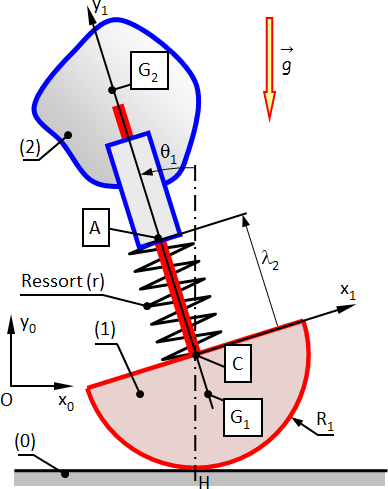
\includegraphics[width=4cm]{fig_01}\\
\textit{Toupie}

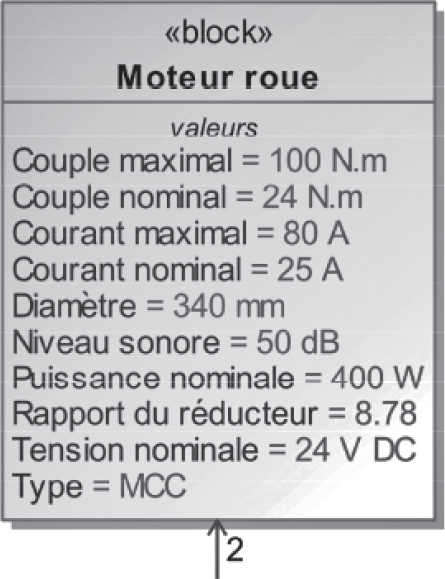
\includegraphics[width=4cm]{fig_02}\\
\textit{Volants d'inertie d'un vilebrequin}

}%figues de la page de garde


\iflivret
\pagestyle{empty}


%%%%%%%% PAGE DE GARDE COURS
\ifcours
% ==== BANDEAU DES TITRES ==== 
\begin{tikzpicture}[remember picture,overlay]
\node at (current page.north west)
{\begin{tikzpicture}[remember picture,overlay]
\node[anchor=north west,inner sep=0pt] at (0,0) {\includegraphics[width=\paperwidth]{\thechapterimage}};
\draw[anchor=west] (-2cm,-8cm) node [line width=2pt,rounded corners=15pt,draw=ocre,fill=white,fill opacity=0.6,inner sep=40pt]{\strut\makebox[22cm]{}};
\draw[anchor=west] (1cm,-8cm) node {\huge\sffamily\bfseries\color{black} %
\begin{minipage}{1cm}
\rotatebox{90}{\LARGE\sffamily\textsc{\color{ocre}\textbf{\xxnumpartie}}}
\end{minipage} \hfill
\begin{minipage}[c]{14cm}
\begin{titrepartie}
\begin{flushright}
\renewcommand{\baselinestretch}{1.1} 
\Large\sffamily\textsc{\textbf{\xxpartie}}
\renewcommand{\baselinestretch}{1} 
\end{flushright}
\end{titrepartie}
\end{minipage} \hfill
\begin{minipage}[c]{3.5cm}
{\large\sffamily\textsc{\textbf{\color{ocre} \discipline}}}
\end{minipage} 
 };
\end{tikzpicture}};
\end{tikzpicture}
% ==== FIN BANDEAU DES TITRES ==== 


% ==== ONGLET 
\begin{tikzpicture}[overlay]
\node[shape=rectangle, 
      rounded corners = .25 cm,
	  draw= ocre,
	  line width=2pt, 
	  fill = ocre!10,
	  minimum width  = 2.5cm,
	  minimum height = 3cm,] at (18.3cm,0) {};
\node at (17.7cm,0) {\rotatebox{90}{\textbf{\Large\color{ocre}{\classe}}}};
%{};
\end{tikzpicture}
% ==== FIN ONGLET 


\vspace{3.5cm}

\begin{tikzpicture}[remember picture,overlay]
\draw[anchor=west] (-2cm,-6cm) node {\huge\sffamily\bfseries\color{black} %
\begin{minipage}{2cm}
\begin{center}
\LARGE\sffamily\textsc{\color{ocre}\textbf{\xxactivite}}
\end{center}
\end{minipage} \hfill
\begin{minipage}[c]{15cm}
\begin{titrechapitre}
\renewcommand{\baselinestretch}{1.1} 
\Large\sffamily\textsc{\textbf{\xxnumchapitre}}

\Large\sffamily\textsc{\textbf{\xxchapitre}}
\vspace{.5cm}

\renewcommand{\baselinestretch}{1} 
\normalsize\normalfont
\xxcompetences
\end{titrechapitre}
\end{minipage}  };
\end{tikzpicture}
\vfill

\begin{flushright}
\begin{minipage}[c]{.3\linewidth}
\begin{center}
\xxfigures
\end{center}
\end{minipage}\hfill
\begin{minipage}[c]{.6\linewidth}
\startcontents
%\printcontents{}{1}{}
\printcontents{}{1}{}
\end{minipage}
\end{flushright}

\begin{tikzpicture}[remember picture,overlay]
\draw[anchor=west] (4.5cm,-.7cm) node {
\begin{minipage}[c]{.2\linewidth}
\begin{flushright}

\includegraphics[width=2cm]{logoCC}
\end{flushright}
\end{minipage}
\begin{minipage}[c]{.2\linewidth}
\textsl{\xxauteur} \\
\textsl{\classe}
\end{minipage}
 };
\end{tikzpicture}

\newpage
\pagestyle{fancy}

%\newpage
%\pagestyle{fancy}

\else
\fi
%% FIN PAGE DE GARDE DES COURS

%%%%%%%% PAGE DE GARDE TD
\iftd
%\begin{tikzpicture}[remember picture,overlay]
%\node at (current page.north west)
%{\begin{tikzpicture}[remember picture,overlay]
%\draw[anchor=west] (-2cm,-3.25cm) node [line width=2pt,rounded corners=15pt,draw=ocre,fill=white,fill opacity=0.6,inner sep=40pt]{\strut\makebox[22cm]{}};
%\draw[anchor=west] (1cm,-3.25cm) node {\huge\sffamily\bfseries\color{black} %
%\begin{minipage}{1cm}
%\rotatebox{90}{\LARGE\sffamily\textsc{\color{ocre}\textbf{\xxnumpartie}}}
%\end{minipage} \hfill
%\begin{minipage}[c]{13.5cm}
%\begin{titrepartie}
%\begin{flushright}
%\renewcommand{\baselinestretch}{1.1} 
%\Large\sffamily\textsc{\textbf{\xxpartie}}
%\renewcommand{\baselinestretch}{1} 
%\end{flushright}
%\end{titrepartie}
%\end{minipage} \hfill
%\begin{minipage}[c]{3.5cm}
%{\large\sffamily\textsc{\textbf{\color{ocre} \discipline}}}
%\end{minipage} 
% };
%\end{tikzpicture}};
%\end{tikzpicture}

%%%%%%%%%% PAGE DE GARDE TD %%%%%%%%%%%%%%%
%\begin{tikzpicture}[overlay]
%\node[shape=rectangle, 
%      rounded corners = .25 cm,
%	  draw= ocre,
%	  line width=2pt, 
%	  fill = ocre!10,
%	  minimum width  = 2.5cm,
%	  minimum height = 2.5cm,] at (18.5cm,0) {};
%\node at (17.7cm,0) {\rotatebox{90}{\textbf{\Large\color{ocre}{\classe}}}};
%%{};
%\end{tikzpicture}

% PARTIE ET CHAPITRE
%\begin{tikzpicture}[remember picture,overlay]
%\draw[anchor=west] (-1cm,-2.1cm) node {\large\sffamily\bfseries\color{black} %
%\begin{minipage}[c]{15cm}
%\begin{flushleft}
%\xxnumchapitre \\
%\xxchapitre
%\end{flushleft}
%\end{minipage}  };
%\end{tikzpicture}

% BANDEAU EXO
\iflivret % SI LIVRET
\begin{tikzpicture}[remember picture,overlay]
\draw[anchor=west] (-2cm,-3.3cm) node {\huge\sffamily\bfseries\color{black} %
\begin{minipage}{5cm}
\begin{center}
\LARGE\sffamily\color{ocre}\textbf{\textsc{\xxactivite}}

\begin{center}
\xxfigures
\end{center}

\end{center}
\end{minipage} \hfill
\begin{minipage}[c]{12cm}
\begin{titrechapitre}
\renewcommand{\baselinestretch}{1.1} 
\large\sffamily\textbf{\textsc{\xxtitreexo}}

\small\sffamily{\textbf{\textit{\color{black!70}\xxsourceexo}}}
\vspace{.5cm}

\renewcommand{\baselinestretch}{1} 
\normalsize\normalfont
\xxcompetences
\end{titrechapitre}
\end{minipage}};
\end{tikzpicture}
\else % ELSE NOT LIVRET
\begin{tikzpicture}[remember picture,overlay]
\draw[anchor=west] (-2cm,-4.5cm) node {\huge\sffamily\bfseries\color{black} %
\begin{minipage}{5cm}
\begin{center}
\LARGE\sffamily\color{ocre}\textbf{\textsc{\xxactivite}}

\begin{center}
\xxfigures
\end{center}

\end{center}
\end{minipage} \hfill
\begin{minipage}[c]{12cm}
\begin{titrechapitre}
\renewcommand{\baselinestretch}{1.1} 
\large\sffamily\textbf{\textsc{\xxtitreexo}}

\small\sffamily{\textbf{\textit{\color{black!70}\xxsourceexo}}}
\vspace{.5cm}

\renewcommand{\baselinestretch}{1} 
\normalsize\normalfont
\xxcompetences
\end{titrechapitre}
\end{minipage}};
\end{tikzpicture}

\fi

\else   % FIN IF TD
\fi


%%%%%%%% PAGE DE GARDE FICHE
\iffiche
\begin{tikzpicture}[remember picture,overlay]
\node at (current page.north west)
{\begin{tikzpicture}[remember picture,overlay]
\draw[anchor=west] (-2cm,-2.25cm) node [line width=2pt,rounded corners=15pt,draw=ocre,fill=white,fill opacity=0.6,inner sep=40pt]{\strut\makebox[22cm]{}};
\draw[anchor=west] (1cm,-2.25cm) node {\huge\sffamily\bfseries\color{black} %
\begin{minipage}{1cm}
\rotatebox{90}{\LARGE\sffamily\textsc{\color{ocre}\textbf{\xxnumpartie}}}
\end{minipage} \hfill
\begin{minipage}[c]{14cm}
\begin{titrepartie}
\begin{flushright}
\renewcommand{\baselinestretch}{1.1} 
\large\sffamily\textsc{\textbf{\xxpartie} \\} 

\vspace{.2cm}

\normalsize\sffamily\textsc{\textbf{\xxnumchapitre -- \xxchapitre}}
\renewcommand{\baselinestretch}{1} 
\end{flushright}
\end{titrepartie}
\end{minipage} \hfill
\begin{minipage}[c]{3.5cm}
{\large\sffamily\textsc{\textbf{\color{ocre} \discipline}}}
\end{minipage} 
 };
\end{tikzpicture}};
\end{tikzpicture}

\iflivret
\begin{tikzpicture}[overlay]
\node[shape=rectangle, 
      rounded corners = .25 cm,
	  draw= ocre,
	  line width=2pt, 
	  fill = ocre!10,
	  minimum width  = 2.5cm,
	  minimum height = 2.5cm,] at (18.5cm,.5cm) {};
\node at (17.9cm,.5cm) {\rotatebox{90}{\textsf{\textbf{\large\color{ocre}{\classe}}}}};
%{};
\end{tikzpicture}
\else
\begin{tikzpicture}[overlay]
\node[shape=rectangle, 
      rounded corners = .25 cm,
	  draw= ocre,
	  line width=2pt, 
	  fill = ocre!10,
	  minimum width  = 2.5cm,
%	  minimum height = 2.5cm,] at (18.5cm,1.1cm) {};
	  minimum height = 2.5cm,] at (18.6cm,0.5cm) {};
\node at (18cm,0.5cm) {\rotatebox{90}{\textsf{\textbf{\large\color{ocre}{\classe}}}}};
%{};
\end{tikzpicture}

\fi

\else
\fi



\else
\pagestyle{empty}


%%%%%%%% PAGE DE GARDE COURS
\ifcours
% ==== BANDEAU DES TITRES ==== 
\begin{tikzpicture}[remember picture,overlay]
\node at (current page.north west)
{\begin{tikzpicture}[remember picture,overlay]
\node[anchor=north west,inner sep=0pt] at (0,0) {\includegraphics[width=\paperwidth]{\thechapterimage}};
\draw[anchor=west] (-2cm,-8cm) node [line width=2pt,rounded corners=15pt,draw=ocre,fill=white,fill opacity=0.6,inner sep=40pt]{\strut\makebox[22cm]{}};
\draw[anchor=west] (1cm,-8cm) node {\huge\sffamily\bfseries\color{black} %
\begin{minipage}{1cm}
\rotatebox{90}{\LARGE\sffamily\textsc{\color{ocre}\textbf{\xxnumpartie}}}
\end{minipage} \hfill
\begin{minipage}[c]{14cm}
\begin{titrepartie}
\begin{flushright}
\renewcommand{\baselinestretch}{1.1} 
\Large\sffamily\textsc{\textbf{\xxpartie}}
\renewcommand{\baselinestretch}{1} 
\end{flushright}
\end{titrepartie}
\end{minipage} \hfill
\begin{minipage}[c]{3.5cm}
{\large\sffamily\textsc{\textbf{\color{ocre} \discipline}}}
\end{minipage} 
 };
\end{tikzpicture}};
\end{tikzpicture}
% ==== FIN BANDEAU DES TITRES ==== 


% ==== ONGLET 
\begin{tikzpicture}[overlay]
\node[shape=rectangle, 
      rounded corners = .25 cm,
	  draw= ocre,
	  line width=2pt, 
	  fill = ocre!10,
	  minimum width  = 2.5cm,
	  minimum height = 3cm,] at (18.3cm,0) {};
\node at (17.7cm,0) {\rotatebox{90}{\textbf{\Large\color{ocre}{\classe}}}};
%{};
\end{tikzpicture}
% ==== FIN ONGLET 


\vspace{3.5cm}

\begin{tikzpicture}[remember picture,overlay]
\draw[anchor=west] (-2cm,-6cm) node {\huge\sffamily\bfseries\color{black} %
\begin{minipage}{2cm}
\begin{center}
\LARGE\sffamily\textsc{\color{ocre}\textbf{\xxactivite}}
\end{center}
\end{minipage} \hfill
\begin{minipage}[c]{15cm}
\begin{titrechapitre}
\renewcommand{\baselinestretch}{1.1} 
\Large\sffamily\textsc{\textbf{\xxnumchapitre}}

\Large\sffamily\textsc{\textbf{\xxchapitre}}
\vspace{.5cm}

\renewcommand{\baselinestretch}{1} 
\normalsize\normalfont
\xxcompetences
\end{titrechapitre}
\end{minipage}  };
\end{tikzpicture}
\vfill

\begin{flushright}
\begin{minipage}[c]{.3\linewidth}
\begin{center}
\xxfigures
\end{center}
\end{minipage}\hfill
\begin{minipage}[c]{.6\linewidth}
\startcontents
%\printcontents{}{1}{}
\printcontents{}{1}{}
\end{minipage}
\end{flushright}

\begin{tikzpicture}[remember picture,overlay]
\draw[anchor=west] (4.5cm,-.7cm) node {
\begin{minipage}[c]{.2\linewidth}
\begin{flushright}

\includegraphics[width=2cm]{logoCC}
\end{flushright}
\end{minipage}
\begin{minipage}[c]{.2\linewidth}
\textsl{\xxauteur} \\
\textsl{\classe}
\end{minipage}
 };
\end{tikzpicture}

\newpage
\pagestyle{fancy}

%\newpage
%\pagestyle{fancy}

\else
\fi
%% FIN PAGE DE GARDE DES COURS

%%%%%%%% PAGE DE GARDE TD
\iftd
%\begin{tikzpicture}[remember picture,overlay]
%\node at (current page.north west)
%{\begin{tikzpicture}[remember picture,overlay]
%\draw[anchor=west] (-2cm,-3.25cm) node [line width=2pt,rounded corners=15pt,draw=ocre,fill=white,fill opacity=0.6,inner sep=40pt]{\strut\makebox[22cm]{}};
%\draw[anchor=west] (1cm,-3.25cm) node {\huge\sffamily\bfseries\color{black} %
%\begin{minipage}{1cm}
%\rotatebox{90}{\LARGE\sffamily\textsc{\color{ocre}\textbf{\xxnumpartie}}}
%\end{minipage} \hfill
%\begin{minipage}[c]{13.5cm}
%\begin{titrepartie}
%\begin{flushright}
%\renewcommand{\baselinestretch}{1.1} 
%\Large\sffamily\textsc{\textbf{\xxpartie}}
%\renewcommand{\baselinestretch}{1} 
%\end{flushright}
%\end{titrepartie}
%\end{minipage} \hfill
%\begin{minipage}[c]{3.5cm}
%{\large\sffamily\textsc{\textbf{\color{ocre} \discipline}}}
%\end{minipage} 
% };
%\end{tikzpicture}};
%\end{tikzpicture}

%%%%%%%%%% PAGE DE GARDE TD %%%%%%%%%%%%%%%
%\begin{tikzpicture}[overlay]
%\node[shape=rectangle, 
%      rounded corners = .25 cm,
%	  draw= ocre,
%	  line width=2pt, 
%	  fill = ocre!10,
%	  minimum width  = 2.5cm,
%	  minimum height = 2.5cm,] at (18.5cm,0) {};
%\node at (17.7cm,0) {\rotatebox{90}{\textbf{\Large\color{ocre}{\classe}}}};
%%{};
%\end{tikzpicture}

% PARTIE ET CHAPITRE
%\begin{tikzpicture}[remember picture,overlay]
%\draw[anchor=west] (-1cm,-2.1cm) node {\large\sffamily\bfseries\color{black} %
%\begin{minipage}[c]{15cm}
%\begin{flushleft}
%\xxnumchapitre \\
%\xxchapitre
%\end{flushleft}
%\end{minipage}  };
%\end{tikzpicture}

% BANDEAU EXO
\iflivret % SI LIVRET
\begin{tikzpicture}[remember picture,overlay]
\draw[anchor=west] (-2cm,-3.3cm) node {\huge\sffamily\bfseries\color{black} %
\begin{minipage}{5cm}
\begin{center}
\LARGE\sffamily\color{ocre}\textbf{\textsc{\xxactivite}}

\begin{center}
\xxfigures
\end{center}

\end{center}
\end{minipage} \hfill
\begin{minipage}[c]{12cm}
\begin{titrechapitre}
\renewcommand{\baselinestretch}{1.1} 
\large\sffamily\textbf{\textsc{\xxtitreexo}}

\small\sffamily{\textbf{\textit{\color{black!70}\xxsourceexo}}}
\vspace{.5cm}

\renewcommand{\baselinestretch}{1} 
\normalsize\normalfont
\xxcompetences
\end{titrechapitre}
\end{minipage}};
\end{tikzpicture}
\else % ELSE NOT LIVRET
\begin{tikzpicture}[remember picture,overlay]
\draw[anchor=west] (-2cm,-4.5cm) node {\huge\sffamily\bfseries\color{black} %
\begin{minipage}{5cm}
\begin{center}
\LARGE\sffamily\color{ocre}\textbf{\textsc{\xxactivite}}

\begin{center}
\xxfigures
\end{center}

\end{center}
\end{minipage} \hfill
\begin{minipage}[c]{12cm}
\begin{titrechapitre}
\renewcommand{\baselinestretch}{1.1} 
\large\sffamily\textbf{\textsc{\xxtitreexo}}

\small\sffamily{\textbf{\textit{\color{black!70}\xxsourceexo}}}
\vspace{.5cm}

\renewcommand{\baselinestretch}{1} 
\normalsize\normalfont
\xxcompetences
\end{titrechapitre}
\end{minipage}};
\end{tikzpicture}

\fi

\else   % FIN IF TD
\fi


%%%%%%%% PAGE DE GARDE FICHE
\iffiche
\begin{tikzpicture}[remember picture,overlay]
\node at (current page.north west)
{\begin{tikzpicture}[remember picture,overlay]
\draw[anchor=west] (-2cm,-2.25cm) node [line width=2pt,rounded corners=15pt,draw=ocre,fill=white,fill opacity=0.6,inner sep=40pt]{\strut\makebox[22cm]{}};
\draw[anchor=west] (1cm,-2.25cm) node {\huge\sffamily\bfseries\color{black} %
\begin{minipage}{1cm}
\rotatebox{90}{\LARGE\sffamily\textsc{\color{ocre}\textbf{\xxnumpartie}}}
\end{minipage} \hfill
\begin{minipage}[c]{14cm}
\begin{titrepartie}
\begin{flushright}
\renewcommand{\baselinestretch}{1.1} 
\large\sffamily\textsc{\textbf{\xxpartie} \\} 

\vspace{.2cm}

\normalsize\sffamily\textsc{\textbf{\xxnumchapitre -- \xxchapitre}}
\renewcommand{\baselinestretch}{1} 
\end{flushright}
\end{titrepartie}
\end{minipage} \hfill
\begin{minipage}[c]{3.5cm}
{\large\sffamily\textsc{\textbf{\color{ocre} \discipline}}}
\end{minipage} 
 };
\end{tikzpicture}};
\end{tikzpicture}

\iflivret
\begin{tikzpicture}[overlay]
\node[shape=rectangle, 
      rounded corners = .25 cm,
	  draw= ocre,
	  line width=2pt, 
	  fill = ocre!10,
	  minimum width  = 2.5cm,
	  minimum height = 2.5cm,] at (18.5cm,.5cm) {};
\node at (17.9cm,.5cm) {\rotatebox{90}{\textsf{\textbf{\large\color{ocre}{\classe}}}}};
%{};
\end{tikzpicture}
\else
\begin{tikzpicture}[overlay]
\node[shape=rectangle, 
      rounded corners = .25 cm,
	  draw= ocre,
	  line width=2pt, 
	  fill = ocre!10,
	  minimum width  = 2.5cm,
%	  minimum height = 2.5cm,] at (18.5cm,1.1cm) {};
	  minimum height = 2.5cm,] at (18.6cm,0.5cm) {};
\node at (18cm,0.5cm) {\rotatebox{90}{\textsf{\textbf{\large\color{ocre}{\classe}}}}};
%{};
\end{tikzpicture}

\fi

\else
\fi



\fi
\setlength{\columnseprule}{.1pt}

\vspace{2cm}
\pagestyle{fancy}
\thispagestyle{plain}



\section{Énoncé du Principe Fondamental de la Dynamique : cas général}

\begin{definition}[Énoncé du Principe Fondamental de la Dynamique]
Soit un ensemble matériel $E$ en mouvement par rapport à un référentiel galiléen ($R_0$), alors la somme des actions mécaniques extérieures s'appliquant sur $E$ est égale au torseur dynamique du mouvement de $E$ par rapport à $R_0$ :

$$
\torseurcin{D}{E}{R_0}=\torseurstat{T}{\overline{E}}{E}.
$$
De plus le \textbf{Principe Fondamental de la Dynamique} postule que pour tout mouvement, il existe au moins un référentiel dans lequel le PFD est vérifié. Ce sera donc un \textbf{référentiel galiléen}.


\begin{minipage}[c]{.48\linewidth}
Le \textbf{torseur dynamique} est de la forme : 
$$
\torseurcin{D}{E}{R_0}=\torseurl{
\vectrd{E}{R_0}=m\;\vectg{G}{E}{R_0}
}{
\vectmd{A}{E}{R_0}
}{A}.
$$

\end{minipage} \hfill
\begin{minipage}[c]{.48\linewidth}
\begin{itemize}
\item On note $\vectrd{S}{R_0}$ la résultante dynamique où l'accélération est \textbf{toujours} calculée au centre d'inertie $G$.
\item Le \textbf{moment dynamique} dépend du point A et se note $\vectmd{A}{E}{R_0}$.
\end{itemize}

\end{minipage} 

%\item On note $\overrightarrow{R_d}(E/R_0)$ la résultante du torseur dynamique : 
%
%$$\overrightarrow{R_d}(S/R_0)=m\;\overrightarrow{a}(G\in E/R_0)
%$$
%\item Le \textbf{moment dynamique} dépend du point A et se note $\vectmd{A}{E}{R_0}$
%\end{itemize}



\end{definition}


Du Principe Fondamental de la dynamique découle plusieurs \textbf{théorèmes généraux}.
\subsection{Théorème de la résultante dynamique}

		\begin{theorem}[Théorème de la résultante dynamique]
			Pour tout ensemble matériel $(E)$ de masse $m$ et de centre d'inertie $G$ en mouvement par rapport à un référentiel galiléen ($R_0$), la somme des résultantes des efforts extérieurs s'appliquant sur $E$ est égale à la résultante dynamique du mouvement de $E$ par rapport à $R_0$ :
$$
\vectf{\bar E}{E}=\vectrd{E}{R_0}=m\;\vectg{G}{E}{R_0}.
$$
	\end{theorem}


%\begin{rem}
%On peut alors définir un Newton comme l'effort à mettre en \oe{}uvre pour mettre en mouvement $\SI{1}{kg}$ avec une accélération de $\SI{1}{m.s^{-2}}$ en son centre de gravité $G$.
%\end{rem}

\subsection{Théorème du moment dynamique}
\begin{theorem}[Théorème du moment dynamique]
			Pour tout ensemble matériel $(E)$ de masse $m$ en mouvement par rapport à un référentiel galiléen ($R_0$), la somme des moments des efforts extérieurs s'appliquant sur $E$ en un point quelconque $A$ est égale au moment dynamique du mouvement de $E$ par rapport à $R_0$ en $A$ :
			$$
				\vectm{A}{\bar E}{E}=\vectmd{A}{E}{R_0}.
			$$
		\end{theorem}

%\begin{exemple}[Application à l'éolienne]
%\question{Déterminer le théorème à utiliser pour relier $C_m$ aux paramètres dynamique du problème.}
%
%\begin{texteCache}
%On pourra appliquer un théorème du moment dynamique s'appliquant sur l'éolienne ($E=\left\{1+2+3\right\}$) en projection sur l'axe $\couple{K}{\overrightarrow{z}_0}$  : 
%
%\begin{align*}
%\moment[K]{\bar E}{E}\cdot \overrightarrow{z}_0=\vDelta[K]{E}{R_0}\cdot \overrightarrow{z}_0.\\
%\\
%\Leftrightarrow\\
%C_m=\left(\vDelta[K]{1}{R_0}+\vDelta[K]{2}{R_0}+\vDelta[K]{3}{R_0}\right)\cdot \overrightarrow{z}_0
%\end{align*}
%\end{texteCache}
%
%\end{exemple}

\section{Torseur cinétique }

\subsection{Définition}
  

%\begin{demonstration}[Résultante cinétique]
%
%\begin{texteCache}
%\begin{align*}
%\overrightarrow{R_c}(S/R_0)=\displaystyle{\int_{P\in S}}\overrightarrow{V}(P/R_0)\;dm=
%\displaystyle{\int_{P\in S}}\left[\frac{d\overrightarrow{OP}}{\dd t}\right]_{R_0}\;dm\\
%=\displaystyle{\int_{P\in S}}\left[\frac{d(\overrightarrow{OG}+\overrightarrow{GP})}{\dd t}\right]_{R_0}\;dm
%=\displaystyle{\int_{P\in S}}\left[\frac{d\overrightarrow{OG}}{\dd t}\right]_{R_0}\;dm+\displaystyle{\int_{P\in S}}\left[\frac{d\overrightarrow{GP}}{\dd t}\right]_{R_0}\;dm.
%\end{align*}
%
%Or, $S$ est à masse conservative,
%
%\begin{align*}
%\displaystyle{\int_{P\in S}}\left[\frac{d\overrightarrow{GP}}{\dd t}\right]_{R_0}\;dm
%=\left[\frac{d}{\dd t}\left(\displaystyle{\int_{P\in S}}\overrightarrow{GP}\;dm\right)\right]_{R_0}=\overrightarrow{0}.
%\end{align*}
%
%On obtient alors,
%
%\begin{align*}
%\overrightarrow{R_c}(S/R_0)=\displaystyle{\int_{P\in S}}\left[\frac{d\overrightarrow{OG}}{\dd t}\right]_{R_0}\;dm
%=\left[\frac{d\overrightarrow{OG}}{\dd t}\right]_{R_0}\displaystyle{\int_{P\in S}}dm\\
%=m\;\overrightarrow{V}(G/R_0)\\
%\end{align*}
%
%\end{texteCache}
%\end{demonstration}

\subsection{Écriture avec l'opérateur d'inertie}

\begin{prop}
Pour un solide $S$ de masse $m$ dans son mouvement par rapport au repère $R_0$ et soit un point $A$ quelconque.
$$\vectmc{A}{S}{R_0}=\inertie{A}{S}\cdot \vecto{S}{R_0}+m\;\vect{AG}\wedge \vectv{A}{S}{R_0}.
$$
%\item \textbf{Dans la pratique}, il faudra utiliser cette formule.
%\end{itemize}
\end{prop}


%\begin{demonstration}
%\begin{texteCache}
%\begin{align*}
%\vSigma[A]{S}{R_0}=\displaystyle{\int_{P\in S}}\overrightarrow{AP}\wedge \overrightarrow{V}(P/R_0)\;dm
%=\displaystyle{\int_{P\in S}}\overrightarrow{AP}\wedge \overrightarrow{V}(P\in S/R_0)\;dm\\
%=\displaystyle{\int_{P\in S}}\overrightarrow{AP}\wedge \left(\overrightarrow{V}(A\in S/R_0)+\overrightarrow{\Omega}(S/R_0)\wedge \overrightarrow{AP}\right)\;dm\\
%=\overline{\overline{I}}_A(S)\cdot \overrightarrow{\Omega}(S/R_0)+M\;\overrightarrow{AG}\wedge \overrightarrow{V}(A\in S/R_0).
%\end{align*}
%\end{texteCache}
%\end{demonstration}

\subsection{Cas particuliers}

\begin{itemize}
\item En appliquant cette formule en un point \textbf{$A$ fixe} dans le mouvement de $S/R_0$, on a :$\vectmc{A}{S}{R_0}=\inertie{A}{S}\cdot \vecto{S}{R_0}$.
\item En appliquant cette formule en \textbf{$G$, centre d'inertie} de $S$, on a :
$
\vectmc{G}{S}{R_0}=\inertie{G}{S}\cdot \vecto{S}{R_0}.
$
\end{itemize}



\subsection{Méthodologie de Calcul}

On considère un ensemble matériel $E$ composé de solides $S_i$. On étudie son mouvement dans le référentiel $R_0$.
On donne la méthodologie de calcul du moment cinétique en un point $A$ sur la figure suivante.%\ref{algo_moment_cine}.

%\begin{figure}[htb]
\begin{center}
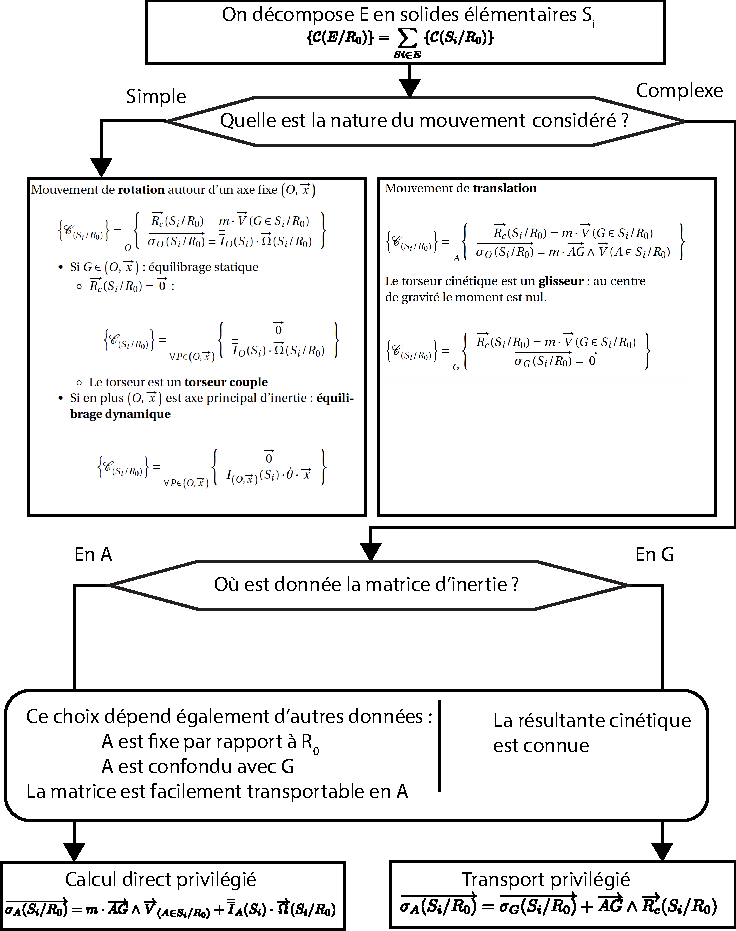
\includegraphics[width=.9\textwidth]{algorigramme_moment_cinetique.pdf}
%\caption{Algorigramme de calcul du moment cinétique \label{algo_moment_cine}}
\end{center}
%\end{figure}

%\begin{exemple}[Application à l'éolienne]
%\question{Déterminer la composante suivant $\overrightarrow{z}_0$ du moment cinétique au point K de la girouette 1 dans son mouvement par rapport au support 0, notée $\overrightarrow{z}_0\cdot \vectmc{K}{1}{0}$.}
%
%\begin{texteCache}
%\begin{itemize}
%\item Le mouvement de $1/0$ est un mouvement de rotation autour d'un axe fixe \couple{K}{\overrightarrow{z}_0} : 
%
%\item $\vectmc{K}{1}{0}\cdot \overrightarrow{z}_0=\left(\overline{\overline{I}}_K(1)\cdot \overrightarrow{\Omega}(1/0)\right)\cdot \overrightarrow{z}_0=\left(\overline{\overline{I}}_K(1)\cdot \dot{\alpha}\cdot \overrightarrow{z}_0 \right)\cdot \overrightarrow{z}_0$
%
%\item or on note J son moment d'inertie par rapport à l'axe \couple{K}{\overrightarrow{z}} soit : 
%\begin{align*}
%\overline{\overline{I}}_K(1)\cdot\overrightarrow{z}_0\cdot \overrightarrow{z}_0=J
%\end{align*}
%
%\item Ainsi : 
%
%\begin{align*}
%\boxed{
%\vectmc{K}{1}{0}\cdot \overrightarrow{z}_0=J\cdot \dot{\alpha}
%}
%\end{align*}
%\end{itemize}
%\end{texteCache}
%
%\question{Déterminer le moment cinétique $\vSigma[K]{2}{0}$  calculé au point K de l'hélice 2 dans son mouvement par rapport à 0.}
%
%\begin{texteCache}
%\begin{itemize}
%\item Le mouvement de $2/0$ n'est pas un mouvement simple. 
%\item On connaît l'opérateur d'inertie en G, on calcule donc : $\vSigma[G]{2}{0}$,
%
%\begin{align*}
%\vSigma[G]{2}{0}=\overline{\overline{I}}_G(2)\cdot \overrightarrow{\Omega}(2/0).
%\end{align*}
%
%\item On calcule $\overrightarrow{\Omega}(2/0)$
%\begin{align*}
%\overrightarrow{\Omega}(2/0)=\overrightarrow{\Omega}(2/1)+\overrightarrow{\Omega}(1/0)=
%\dot{\beta}\cdot \overrightarrow{x}_{1,2}+\dot{\alpha}\cdot \overrightarrow{z}_{1}
%\\=\dot{\beta}\cdot \overrightarrow{x}_{1,2}
%+\dot{\alpha}\left(\cos\beta\overrightarrow{z}_2+\sin\beta\overrightarrow{y}_2\right)\\
%\end{align*}
%
%\item On calcule $\vSigma[G]{2}{0}$ : 
%
%\begin{align*}
%\vSigma[G]{2}{0}=\left(
%\begin{array}{ccc}
%A & 0 & 0 \\ 
%0 & B & 0 \\ 
%0 & 0 & C
%\end{array}
%\right)_{\triplet{\overrightarrow{x}_2}{\overrightarrow{y}_2}{\overrightarrow{z}_2}} \cdot 
%\left(
%\begin{array}{c}
%\dot{\beta}\\
%\dot{\alpha}\cdot \sin\beta\\
%\dot{\alpha}\cdot \cos\beta\\
%\end{array}
%\right)_{\triplet{\overrightarrow{x}_2}{\overrightarrow{y}_2}{\overrightarrow{z}_2}}\\
%=\left(
%\begin{array}{c}
%A\cdot \dot{\beta}\\
%B\cdot \dot{\alpha}\cdot \sin\beta\\
%C\cdot \dot{\alpha}\cdot \cos\beta\\
%\end{array}
%\right)_{\triplet{\overrightarrow{x}_2}{\overrightarrow{y}_2}{\overrightarrow{z}_2}}\\
%\end{align*}
%\end{itemize}
%\end{texteCache}
%\end{exemple}

%\setcounter{cptExemple}{2}
%\begin{exemple}[Application à l'éolienne]
%\begin{texteCache}
%\begin{itemize}
%\item On calcule $\vSigma[K]{2}{0}$ : 
%
%\begin{itemize}
%\item \begin{align*}
%\vSigma[K]{2}{0}=\vSigma[G]{2}{0}+\overrightarrow{KG}\wedge \overrightarrow{R_c}(2/0)
%=\vSigma[G]{2}{0}+a\cdot \overrightarrow{x}_1\wedge M\cdot \overrightarrow{V}(G\in 2/0)
%\end{align*}
%
%\item On calcule $\overrightarrow{V}(G\in 2/0)$ : 
%
%\begin{align*}
%\overrightarrow{V}(G\in 2/0)=\overrightarrow{V}(K\in 2/0)+\overrightarrow{GK}\wedge \overrightarrow{\Omega}(2/0)=
%\overrightarrow{0}-a\cdot \overrightarrow{x}_1\wedge \left(\dot{\beta}\cdot \overrightarrow{x}_{1,2}+\dot{\alpha}\cdot \overrightarrow{z}_{1}\right)\\
%=a\cdot \dot{\alpha}\overrightarrow{y}_{1} 
%\end{align*}
%
%\item On calcule $a\cdot \overrightarrow{x}_1\wedge M\cdot \overrightarrow{V}(G\in 2/0)$ : 
%
%\begin{align*}
%a\cdot \overrightarrow{x}_1\wedge M\cdot \overrightarrow{V}(G\in 2/0)=
%a\cdot \overrightarrow{x}_1\wedge M\left(a\cdot \dot{\alpha}\overrightarrow{y}_{1} \right)=\\
%M\cdot a^2\cdot \dot{\alpha}\cdot \overrightarrow{z}_1
%\end{align*}
%
%\item On en déduit $\vSigma[K]{2}{0}$: 
%
%\begin{align*}
%\vSigma[K]{2}{0}=\left(
%\begin{array}{c}
%A\cdot \dot{\beta}\\
%B\cdot \dot{\alpha}\cdot \sin\beta+M\cdot a^2\cdot \dot{\alpha}\sin\beta\\
%C\cdot \dot{\alpha}\cdot \cos\beta+M\cdot a^2\cdot \dot{\alpha}\cos\beta\\
%\end{array}
%\right)_{\triplet{\overrightarrow{x}_2}{\overrightarrow{y}_2}{\overrightarrow{z}_2}}\\
%\end{align*}
%
%\end{itemize}
%
%\end{itemize}
%\end{texteCache}
%
%\question{Déterminer le moment cinétique $\vSigma[K]{3}{0}$.}
%
%\begin{texteCache}
%\begin{itemize}
%\item Le solide $3$ est solide à masse ponctuelle, ainsi $\vSigma[Q]{3}{0}=\overrightarrow{0}$.
%\item $\vSigma[K]{3}{0}=\overrightarrow{KQ}\wedge m\cdot \overrightarrow{V}(Q\in 3/0)$ : 
%\begin{itemize}
%\item On calcule $\overrightarrow{KQ}$ : 
%\begin{align*}
%\overrightarrow{KQ}=\overrightarrow{KG}+\overrightarrow{GQ}=a\cdot \overrightarrow{x}_1-b\cdot \overrightarrow{z}_2
%\end{align*}
%\item On calcule $\overrightarrow{V}(Q\in 3/0)$ : 
%
%\begin{align*}
%\overrightarrow{V}(Q\in 3/0)=\overrightarrow{V}(Q\in 3/2)+\overrightarrow{V}(Q\in 2/1)+\overrightarrow{V}(Q\in 1/0)
%\\
%=\overrightarrow{0}+\overrightarrow{V}(G\in 2/1)+\overrightarrow{QG}\wedge \overrightarrow{\Omega}(2/1)
%+\overrightarrow{V}(G\in 1/0)+\overrightarrow{QG}\wedge \overrightarrow{\Omega}(1/0)\\
%=\overrightarrow{0}+b\cdot \overrightarrow{z}_2\wedge \dot{\beta}\cdot \overrightarrow{x}_2+ a\cdot \dot{\alpha}\cdot \overrightarrow{y}_1+b\cdot \overrightarrow{z}_2\wedge \dot{\alpha}\cdot \overrightarrow{z}_1\\
%=b\cdot \dot{\beta}\cdot \overrightarrow{y}_2+a\cdot \dot{\alpha}\cdot \overrightarrow{y}_1-b\cdot\dot{\alpha} \sin\beta\cdot \overrightarrow{x}_{1,2}
%\end{align*}
%
%\item On calcule $\overrightarrow{KQ}\wedge m\overrightarrow{V}(Q\in 3/0)$ : 
%
%\begin{align*}
%\overrightarrow{KQ}\wedge m\overrightarrow{V}(Q\in 3/0)=m\cdot \left[a\cdot \overrightarrow{x}_1-b\cdot \overrightarrow{z}_2\right]\wedge\left[b\cdot \dot{\beta}\cdot \overrightarrow{y}_2+a\cdot \dot{\alpha}\cdot \overrightarrow{y}_1-b\cdot\dot{\alpha} \sin\beta\cdot \overrightarrow{x}_{1,2}\right]\\
%=m\left[a\cdot b\cdot \overrightarrow{z}_2+a^2\cdot \dot{\alpha}\cdot\overrightarrow{z}_1+b^2\cdot \dot{\beta}\cdot\overrightarrow{x}_2+b\cdot a\cdot \dot{\alpha}\cdot \cos\beta\cdot \overrightarrow{x}_1+b^2\cdot \dot{\alpha}\sin\beta\cdot \overrightarrow{y}_2\right]
%\end{align*}
%\end{itemize}
%
%\item,
%
%\begin{align*}
%\boxed{
%\vSigma[K]{3}{0}=m\left[a\cdot b\cdot\dot{\beta} \overrightarrow{z}_2+a^2\cdot \dot{\alpha}\cdot\overrightarrow{z}_1+b^2\cdot \dot{\beta}\cdot\overrightarrow{x}_2+b\cdot a\cdot \dot{\alpha}\cdot \cos\beta\cdot \overrightarrow{x}_1+b^2\cdot \dot{\alpha}\sin\beta\cdot \overrightarrow{y}_2\right]
%}
%\end{align*}
%\end{itemize}
%
%\end{texteCache}
%\end{exemple}


\section{Torseur dynamique}
\subsection{Définition}
\begin{definition}%[Torseur dynamique]
Le \textbf{torseur dynamique} d'un solide $S$ dans son mouvement par rapport à $R_0$ se définit de la façon suivante,

$$
\torseurcin{D}{S}{R_0}=\torseurl{\overrightarrow{R_d}(S/R_0)=\displaystyle{\int_{P\in S}}\overrightarrow{\Gamma}(P/R_0)\;\dd m}{\vectmd{A}{S}{R_0}=\displaystyle{\int_{P\in S}}\overrightarrow{AP}\wedge \overrightarrow{\Gamma}(P/R_0)\;\dd m}{A}
$$

\begin{itemize}
\item La résultante du torseur dynamique, $\overrightarrow{R_d}(S/R_0)$ ne dépend pas du point $A$ mais uniquement du centre de gravité $G$ de S (de masse $m$) et vérifie :

$$\overrightarrow{R_d}(S/R_0)=m\;\overrightarrow{\Gamma}(G/R_0).
$$
\item Le moment dynamique dépend du point A et peut s'exprimer avec la formule fondamentale de changement de point :
$$
\vectmd{B}{S}{R_0}=\vectmd{A}{S}{R_0}+\overrightarrow{BA}\wedge \overrightarrow{R_d}(S/R_0).
$$
\end{itemize}

\end{definition}


%\begin{demonstration}[Résultante dynamique]

%\begin{texteCache}
%\begin{align*}
%\overrightarrow{R_d}(S/R_0)=\displaystyle{\int_{P\in S}}\overrightarrow{a}(P/R_0)\;dm=
%\displaystyle{\int_{P\in S}}\left[\frac{d^2\overrightarrow{OP}}{dt^2}\right]_{R_0}\;dm\\
%=\displaystyle{\int_{P\in S}}\left[\frac{d^2(\overrightarrow{OG}+\overrightarrow{GP})}{dt^2}\right]_{R_0}\;dm
%=\displaystyle{\int_{P\in S}}\left[\frac{d^2\overrightarrow{OG}}{dt^2}\right]_{R_0}\;dm+\displaystyle{\int_{P\in S}}\left[\frac{d^2\overrightarrow{GP}}{dt^2}\right]_{R_0}\;dm.
%\end{align*}
%
%Or, $S$ est à masse conservative,
%
%\begin{align*}
%\displaystyle{\int_{P\in S}}\left[\frac{d^2\overrightarrow{GP}}{dt^2}\right]_{R_0}\;dm
%=\left[\frac{d^2}{dt^2}\left(\displaystyle{\int_{P\in S}}\overrightarrow{GP}\;dm\right)\right]_{R_0}=\overrightarrow{0}.
%\end{align*}
%
%On obtient alors,
%
%\begin{align*}
%\overrightarrow{R_d}(S/R_0)=\displaystyle{\int_{P\in S}}\left[\frac{d^2\overrightarrow{OG}}{dt^2}\right]_{R_0}\;dm
%=\left[\frac{d^2\overrightarrow{OG}}{dt^2}\right]_{R_0}\displaystyle{\int_{P\in S}}dm\\
%=m\;\overrightarrow{a}(G/R_0)\\
%\end{align*}
%
%\end{texteCache}
%\end{demonstration}

\subsection{Relations entre les torseurs cinétiques et dynamiques}
\begin{prop}[Relations entre les torseurs cinétiques et dynamiques]
Pour un solide S de masse $M$ dans son mouvement par rapport au repère $R_0$ et soit un point $A$ quelconque.
\begin{itemize}
\item Relation entre les \textbf{résultantes} :

$$
\overrightarrow{R_d}(S/R_0)=\left[\frac{\dd \overrightarrow{R_c}(S/R_0)}{\dd t}\right]_{R_0}.
$$
\item Relation entre les \textbf{moments} :

$$
\vectmd{A}{S}{R_0}=\left[\frac{\dd \vectmc{A}{S}{R_0}}{\dd t}\right]_{R_0}+\overrightarrow{V(A/R_0)}\wedge \overrightarrow{R_c}(S/R_0).
$$
\end{itemize}
\end{prop}




\subsection{Cas particuliers}

%\begin{rem}
\begin{itemize}
\item En appliquant cette formule en un point \textbf{$O$ fixe} dans $R_0$, on a :

$$
\vectmd{O}{S}{R_0}=\left[\frac{\dd \vectmc{O}{S}{R_0}}{\dd t}\right]_{R_0}.
$$
\item En appliquant cette formule en un point \textbf{$G$, centre d'inertie de $S$}, on a :

$$
\vectmd{G}{S}{R_0}=\left[\frac{\dd \vectmc{G}{S}{R_0}}{\dd t}\right]_{R_0}.
$$

\end{itemize}
%\end{rem}





\newpage
\subsection{Méthodologie de calcul}

On considère un ensemble matériel $E$ composé de solides $S_i$. On étudie son mouvement dans le référentiel $R_0$.
On donne l'algorigramme de calcul du moment dynamique en un point $A$ sur la figure ci-dessous.%\ref{algo_moment_dyna}.

%\begin{exemple}[Application à l'éolienne]
%\question{Déterminer la composante suivant $\overrightarrow{z}_0$ du moment dynamique au point K de la girouette 1 dans son mouvement par rapport au support 0, notée $\overrightarrow{z}_0\cdot \vDelta[K]{1}{0}$.}
%
%\begin{texteCache}
%\begin{align*}
%\overrightarrow{z}_0\cdot \vDelta[K]{1}{0}=\overrightarrow{z}_0\cdot\left[\frac{d\vSigma[K]{1}{0}}{\dd t}\right]_{R_0}
%=\left[\frac{d\overrightarrow{z}_0\cdot\vSigma[K]{1}{0}}{\dd t}\right]_{R_0}=J\cdot \ddot{\alpha}
%\end{align*}
%\end{texteCache}
%
%\question{Déterminer la composante suivant $\overrightarrow{z}_0$ du moment dynamique $\overrightarrow{z}_0\cdot \vDelta[K]{2}{0}$.}
%
%\begin{texteCache}
%\begin{align*}
%\overrightarrow{z}_0\cdot \vDelta[K]{2}{0}=\overrightarrow{z}_0\cdot\left[\frac{d\vSigma[K]{2}{0}}{\dd t}\right]_{R_0}
%=\left[\frac{d\overrightarrow{z}_0\cdot\vSigma[K]{2}{0}}{\dd t}\right]_{R_0}
%\end{align*}
%
%Or, $\overrightarrow{z}_{0,1}=\cos\beta\cdot \overrightarrow{z}_2+\sin\beta\cdot \overrightarrow{y}_2$,
%
%\begin{align*}
%\overrightarrow{z}_0\cdot\vSigma[K]{2}{0}=
%\left(
%\begin{array}{c}
%A\cdot \dot{\beta}\\
%B\cdot \dot{\alpha}\cdot \sin\beta+M\cdot a^2\cdot \dot{\alpha}\sin\beta\\
%C\cdot \dot{\alpha}\cdot \cos\beta+M\cdot a^2\cdot \dot{\alpha}\cos\beta\\
%\end{array}
%\right)_{\triplet{\overrightarrow{x}_2}{\overrightarrow{y}_2}{\overrightarrow{z}_2}}
%\cdot
%\left(
%\begin{array}{c}
%0\\
%\sin\beta\\
%\cos\beta\\
%\end{array}
%\right)_{\triplet{\overrightarrow{x}_2}{\overrightarrow{y}_2}{\overrightarrow{z}_2}}
%\\
%=\dot{\alpha}\left[B\cdot \sin^2\beta+C\cdot \cos^2\beta+M\cdot a^2\right]
%\end{align*}
%
%d'où,
%\begin{align*}
%\boxed{
%\overrightarrow{z}_0\cdot \vDelta[K]{2}{0}=\ddot{\alpha}\left[B\cdot \sin^2\beta+C\cdot \cos^2\beta+M\cdot a^2\right]
%+2\cdot\dot{\alpha}\dot{\beta}\cdot \cos\beta\cdot \sin\beta\left[B-C\right].
%}
%\end{align*}
%
%\end{texteCache}
%
%\question{Déterminer la projection du moment dynamique de $3/0$ selon $\overrightarrow{z}_0$ : $\overrightarrow{z}_0\cdot \vSigma[K]{3}{0}$.}
%
%
%
%\begin{texteCache}
%\begin{minipage}{0.5\textwidth}
%\begin{center}
%\scFigCalc[x_{1,2}]{y_1}{z_1}{y_2}{z_2}{\beta}
%\end{center}
%\end{minipage}
%\begin{minipage}{0.5\textwidth}
%\begin{align*}
%\overrightarrow{z}_{0,1}\cdot \overrightarrow{z}_2=\cos\beta\\
%\overrightarrow{z}_{0,1}\cdot \overrightarrow{z}_1=1\\
%\overrightarrow{z}_{0,1}\cdot \overrightarrow{x}_0=0\\
%\overrightarrow{z}_{0,1}\cdot \overrightarrow{x}_1=0\\
%\overrightarrow{z}_1\cdot \overrightarrow{y}_2=\sin\beta\\
%\end{align*}
%\end{minipage}
%
%On trouve alors : 
%
%\begin{align*}
%\overrightarrow{z}_0\cdot \vSigma[K]{3}{0}=
%m\frac{d\left[a\cdot b\cdot \dot{\beta}\cos\beta+a^2\cdot \dot{\alpha}+b^2\cdot \dot{\alpha}\sin^2\beta\right]}{\dd t}\\
%=m\left[a\cdot b\cdot \left(\ddot{\beta}\cos\beta-\dot{\beta}^2\sin\beta\right)+a^2\ddot{\alpha}+b^2\cdot\left(\ddot{\alpha}\sin^2\beta+2\dot{\alpha}\dot{\beta}\sin\beta\cos\beta\right)\right]
%\end{align*}
%
%\end{texteCache}
%
%\question{Dans le cas d'une vitesse de rotation de l'hélice 2 ($\dot{\beta}$) constante et dans le cas où l'angle $\alpha$ est constant (pas de changement d'orientation de l'éolienne) déterminer l'expriment du couple $C_m$ que devrait fournir un moteur placé dans le mat (entre 0 et 1) pour "contrer" les effets dynamiques du balourd.}
%
%\begin{texteCache}
%Le théorème du moment dynamique autour de l'axe $\couple{K}{\overrightarrow{z}_{0,1}}$ donne :
%
%\begin{align*}
%C_m=-m\cdot a\cdot b\cdot \dot{\beta}^2\sin\beta
%\end{align*} 
%
%
%\end{texteCache}
%\end{exemple}

%\begin{figure}[htb]
\begin{center}
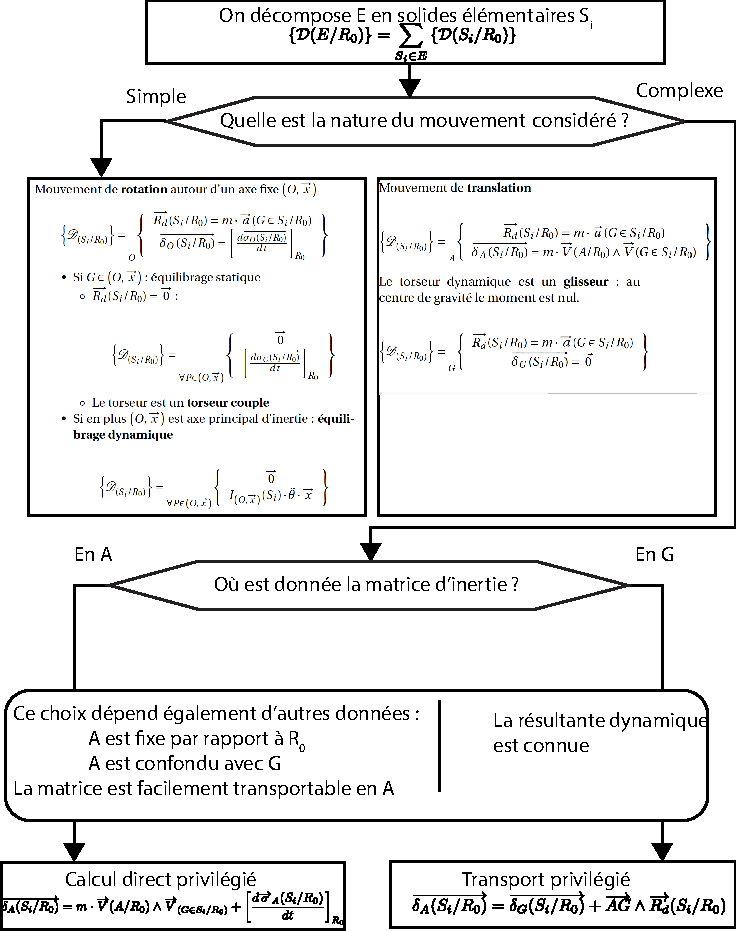
\includegraphics[width=.9\textwidth]{algorigramme_moment_dynamique.pdf}
%\caption{Algorigramme de calcul du moment dynamique \label{algo_moment_dyna}}
\end{center}
%\end{figure}


\begin{thebibliography}{2}
   \bibitem[1]{ref1} Emilien Durif, {\it Cinétique des solides, Lycée La Martinière Monplaisir, Lyon.}
      \bibitem[2]{ref2} Florestan Mathurin, {\it Cinétique, Lycée Bellevue, Toulouse, \url{http://florestan.mathurin.free.fr/}.}
%      \bibitem[3]{ref3} Robert Papanicola, {\it Opérateurs d'inetie, Lycée Charlemagne, Paris, \url{http://sciences-indus-cpge.papanicola.info/}.}
\end{thebibliography}

\newpage

\section*{Bilan}
\footnotesize
\begin{center}
\rotatebox{90}{
\begin{tabular}{|c|c|c|c|}
\hline
Point considéré & Point quelconque $A$ & Centre de gravité $G$  & Point fixe dans $\mathcal{R}_0$ $A$  \\
\hline
&&& \\
Torseur cinétique$\torseurcin{C}{S}{R_0}$
& 
$\torseurl{
\overrightarrow{R_c}(S/R_0)=m\;\overrightarrow{V}(G/R_0)
}{\vectmc{A}{S}{R_0}=\inertie{A}{S}\cdot \vecto{S}{R_0}+m\;\vect{AG}\wedge \vectv{A}{S}{R_0}
}{A}$ 
&
$\torseurl{
\overrightarrow{R_c}(S/R_0)=m\;\overrightarrow{V}(G/R_0)
}{
\vectmc{G}{S}{R_0}=\inertie{G}{S}\cdot \vecto{S}{R_0}
}{G}$
&
$\torseurl{
\overrightarrow{R_c}(S/R_0)=m\;\overrightarrow{V}(G/R_0)
}{
\vectmc{A}{S}{R_0}=\inertie{A}{S}\cdot \vecto{S}{R_0}
}{A}$
\\
&&& \\ \hline
&&& \\
Torseur dynamique $
\torseurcin{D}{S}{R_0}$ & 
$
\torseurl{
\overrightarrow{R_d}(S/R_0)=m\;\overrightarrow{\Gamma}(G/R_0)
}{
\vectmd{A}{S}{R_0}=\left[\frac{\dd \vectmc{A}{S}{R_0}}{\dd t}\right]_{R_0}+\overrightarrow{V(A/R_0)}\wedge \overrightarrow{R_c}(S/R_0)
}{A}
$
&
$
\torseurl{
\overrightarrow{R_d}(S/R_0)=m\;\overrightarrow{\Gamma}(G/R_0)
}{
\vectmd{G}{S}{R_0}=\left[\frac{\dd \vectmc{G}{S}{R_0}}{\dd t}\right]_{R_0}
}{G}
$
&
$
\torseurl{
\overrightarrow{R_d}(S/R_0)=m\;\overrightarrow{\Gamma}(G/R_0)
}{
\vectmd{A}{S}{R_0}=\left[\frac{\dd \vectmc{A}{S}{R_0}}{\dd t}\right]_{R_0}
}{A}
$
\\ 
&&& \\ \hline
\end{tabular}}

\end{center}


\normalsize



%% Activation Barriere
\renewcommand{\td}{Cy_04_02_Activation_01_Barrirere}
%% Sujet Normal par défaut
\newpage
\fichetrue \proffalse \tdtrue \coursfalse \normaltrue \difficilefalse \tdifficilefalse \collefalse
\graphicspath{{../../style/png/}{../../\chap/\td/images/}}
\input{../../\chap/\td/\td.tex}

%% Sujet colle (TO DO)
%\newpage
%\fichetrue \proffalse \tdtrue \coursfalse \normaltrue \difficilefalse \tdifficilefalse \colletrue
%\graphicspath{{../../style/png/}{../../\chap/\td/images/}}
%\input{../../Chapitre_01_Correction/\td/\td.tex}

%% Sujet Corrigé
\newpage
\fichetrue \proftrue \tdtrue \coursfalse \normaltrue \difficilefalse  \tdifficilefalse \collefalse
\graphicspath{{../../style/png/}{../../\chap/\td/images/}}
\input{../../\chap/\td/\td.tex}

%% Application Vilebrequin
\renewcommand{\td}{Cy_04_02_Application_01_Vilebrequin}
%% Sujet Normal par défaut
\newpage
\fichetrue \proffalse \tdtrue \coursfalse \normaltrue \difficilefalse \tdifficilefalse \collefalse
\graphicspath{{../../style/png/}{../../\chap/\td/images/}}
\input{../../\chap/\td/\td.tex}

%%  Corrigé
\newpage
\fichetrue \proftrue \tdtrue \coursfalse \normaltrue \difficilefalse  \tdifficilefalse \collefalse
\graphicspath{{../../style/png/}{../../\chap/\td/images/}}
\input{../../\chap/\td/\td.tex}


%% Application triaxe
\renewcommand{\td}{Cy_04_02_Application_02_Triaxe}
%% Sujet Normal par défaut
\newpage
\fichetrue \proffalse \tdtrue \coursfalse \normaltrue \difficilefalse \tdifficilefalse \collefalse
\graphicspath{{../../style/png/}{../../\chap/\td/images/}}
\input{../../\chap/\td/\td.tex}

%%  Corrigé
\newpage
\fichetrue \proftrue \tdtrue \coursfalse \normaltrue \difficilefalse  \tdifficilefalse \collefalse
\graphicspath{{../../style/png/}{../../\chap/\td/images/}}
\input{../../\chap/\td/\td.tex}

\end{document}



